%% Modified by Abdullah Khanfor for Stevens Institute of Technology PhD thesis format design guidelines 2019-2020
% NYU PhD thesis format. Original template created by José Koiller 2007--2008.
%% Updated by Anshul Vikram Pandey with new design guidelines. 2017-2018

%% Use the first of the following lines during production to
%% easily spot "overfull boxes" in the output. Use the second
%% line for the final version.
% \documentclass[12pt,draft,letterpaper]{report}
% \documentclass[12pt,letterpaper]{report}
\documentclass[12pt]{report}

%% Replace the title, name, advisor name, graduation date and dedication below with
%% your own. Graduation months must be January, May or September.
\newcommand{\thesistitle}{TITLE TO JUSTIFY YOUR PHD YEARS}
\newcommand{\thesisauthor}{Your Name}
\newcommand{\thesisadvisor}{Your Advisor's Name}
\newcommand{\thesisyear}{2020}
\newcommand{\thesisname}{Abdullah Khanfor}
\newcommand{\thesischairadvisor}{Dr. }    % this name prints on the title page as chairman and the abstract page as advisor
\newcommand{\committeenameA}{Dr. }
\newcommand{\committeenameB}{Dr. }
\newcommand{\committeenameC}{Dr. }
\newcommand{\thesisdepartment}{Systems Engineering}
\newcommand{\thesisdate}{November 22, 2020}
\newcommand{\thesistype}{dissertation}
\newcommand{\thesisdegree}{Doctor of Philosophy}
\newcommand{\graddate}{\the\year} % like 2020, 2019, no month or day should be written
\newcommand{\thesissigline}[1]{%
  \leftline{\hbox to 2.5in{}\hrulefill}
  \endgraf
  \vspace*{-18pt}
  \leftline{\hbox to 2.53in{}{#1}}}

%% If you do not want a dedication, scroll down and comment out
%% the appropriate lines in this file.
\newcommand{\thesisdedication}{To all the Ph.D. pursuing brave souls}

%% The following makes chapters and sections, but not subsections,
%% appear in the TOC (table of contents). Increase to 2 or 3 to
%% make subsections or subsubsections appear, respectively. It seems
%% to be usual to use the "1" setting, however.
\setcounter{tocdepth}{1}

%% Sectional units up to subsubsections are numbered. To number
%% subsections, but not subsubsections, decrease this counter to 2.
\setcounter{secnumdepth}{3}

% Setting a gap between page number and text block

%% This inputs your auxiliary file with \usepackage's and \newcommand's:
%% It is assumed that that file is called "definitions.tex".
%%
%% Place here your \usepackage's. Some recommended packages are already included.
%%

% Graphics:
\usepackage[final]{graphicx}
%\usepackage{graphicx} % use this line instead of the above to suppress graphics in draft copies
%\usepackage{graphpap} % \defines the \graphpaper command

% Indent first line of each section:
%\usepackage{indentfirst}

% Good AMS stuff:
\usepackage{amsthm} % facilities for theorem-like environments
\usepackage[tbtags]{amsmath} % a lot of good stuff!

% Fonts and symbols:
\usepackage{amsfonts}
\usepackage{amssymb}

\usepackage{xspace}
\usepackage{algorithmic}
\usepackage{algorithm}
\usepackage{microtype}
\usepackage{subfigure}
\usepackage{color}
\usepackage{todonotes}
\usepackage{url}
\newfloat{algorithm}{t}{lop}

\usepackage{blindtext}

%% Controls spacing between lines (\doublespacing, \onehalfspacing, etc.):
\usepackage[utf8x]{inputenc}
\usepackage{fancyhdr}

% This package to change the font if the document. This font is optional as you preference. You can comment it to use the CMU font
%\usepackage{helvet}
%\renewcommand{\familydefault}{\sfdefault}

%% \usepackage{amsmath}
%% \usepackage{amssymb}
\usepackage{lipsum}
% \newfloat{algorithm}{t}{lop}

% Packages for setting the length and width of document
\usepackage{setspace}

% Package for sideway images and figures
\usepackage{rotating}
\usepackage{pdflscape}

% Formatting tools:
%\usepackage{relsize} % relative font size selection, provides commands \textsmalle, \textlarger
%\usepackage{xspace} % gentle spacing in macros, such as \newcommand{\acims}{\textsc{acim}s\xspace}

% Page formatting utility:
%\usepackage{geometry}
\usepackage{multirow}

\usepackage{listings}

% For citations
\usepackage[numbers,sort]{natbib}
\usepackage[nottoc]{tocbibind}

\usepackage[all,cmtip]{xy}

% Change the color of the hyperlinks and titles from blue to black
\usepackage{hyperref}
\hypersetup{
    colorlinks = false,
    linkbordercolor = {white},
    linkcolor=black,
    filecolor=black,
    urlcolor=black,
    citecolor=black
}

%%
%% Place here your \newcommand's and \renewcommand's. Some examples already included.
%%
%\newcommand{\acims}{\textsc{acim}s\xspace}
\newcommand{\Mspace}        {{\mathbb M}}
\newcommand{\Rspace}        {{\mathbb R}}
\newcommand{\Cspace}        {{\mathbb C}}

\newcommand{\Mo}        {{\hat M}}
\newcommand{\Ms}        {{\tilde M}}
\newcommand{\Do}          {{\hat D}}
\newcommand{\Ds}        {{\tilde D}}
\newcommand{\doo}          {{\hat d}}
\newcommand{\dss}        {{\tilde d}}
\newcommand{\w}        {{\mathbf w}}

% general
\newcommand{\ie}{i.e.}
\newcommand{\eg}{e.g.}
\newcommand{\reffig}[1]{{Figure~\ref{#1}}}
\newcommand{\refchap}[1]{{Chapter~\ref{#1}}}
\newcommand{\refsec}[1]{{Section~\ref{#1}}}
\newcommand{\reftab}[1]{{Table~\ref{#1}}}
\newcommand{\refapp}[1]{{Appendix~\ref{#1}}}
\newcommand{\refeq}[1]{{Equation~\ref{#1}}}
\newcommand{\refalg}[1]{{Algorithm~\ref{#1}}}
\newcommand{\myparagraph}[1]{\noindent \textbf{#1}}
\newcommand{\highlight}[1]{{\color{black}#1}}

%%
%% Place here your \newtheorem's:
%%

%% Some examples commented out below. Create your own or use these...
%%%%%%%%%\swapnumbers % this makes the numbers appear before the statement name.
%\theoremstyle{plain}
%\newtheorem{thm}{Theorem}[chapter]
%\newtheorem{prop}[thm]{Proposition}
%\newtheorem{lemma}[thm]{Lemma}
%\newtheorem{cor}[thm]{Corollary}

%\theoremstyle{definition}
%\newtheorem{define}{Definition}[chapter]

%\theoremstyle{remark}
%\newtheorem*{rmk*}{Remark}
%\newtheorem*{rmks*}{Remarks}

%% This defines the "proo" environment, which is the same as proof, but
%% with "Proof:" instead of "Proof.". I prefer the former.
%\newenvironment{proo}{\begin{proof}[Proof:]}{\end{proof}}

%\usepackage[subfigure]{tocloft}
\usepackage[explicit]{titlesec}%
\usepackage{titletoc}
\usepackage{etoolbox}

% To add space between the Table of Contents, List of Figures and the List of Tables and the list content
\addtocontents{toc}{\vspace{1.2cm}}
\addtocontents{lof}{\vspace{1.2cm}}
\addtocontents{lot}{\vspace{1.2cm}}

% This command for chapters
\newcommand\chap[1]{%
  \chapter*{#1}%
  \addcontentsline{toc}{chapter}{#1}}

% Table of contents formatting
% Removing the dots between the Title and the page number
\makeatletter
\renewcommand{\@dotsep}{10000} 
\makeatother

\usepackage{tabto}
\usepackage{makebox}

% Table of contents font and space modifications

\titlecontents{chapter}[0pt]
    {\vskip 10pt \bfseries}
    {\bfseries\text{Chapter }\thecontentslabel\tabto{3.5cm}}
    {}
    {\hfill\bfseries\contentspage}

\titlecontents{section}[0pt]
    {}
    {\quad\quad\thecontentslabel\tabto{3.5cm}}
    {}
    {\hfill\contentspage}

\titlecontents{subsection}[0pt]
    {}
    {\quad\quad\thecontentslabel\tabto{3.5cm}}
    {}
    {\hfill\contentspage}
    
\titlecontents{table}[0pt]
    {}
    {\quad\quad\thecontentslabel\tabto{3.5cm}}
    {}
    {\hfill\contentspage}

\titlecontents{figure}[0pt]
    {}
    {\quad\quad\thecontentslabel\tabto{3.5cm}}
    {}
    {\hfill\contentspage}

% Change the Table of Contents, List of Tables ... etc. font size insited of big font
\renewcommand{\contentsname}{\normalsize{Table of Contents}}
\renewcommand{\listfigurename}{\normalsize{List of Figures}}
\renewcommand{\listtablename}{\normalsize{List of Tables}}
\renewcommand{\bibname}{\normalsize{Bibliography}}
\renewcommand{\indexname}{\normalsize{Index}}

% May 2009 added this to move page number up a bit
\addtolength{\voffset}{-2em}

% This is to format the chapter tags in this file
\usepackage{chngcntr}
\usepackage{lipsum}% just to generate text for the example

%% Page layout (customized to letter paper and Stevens requirements):
% if not using pdflatex to produce output, you may need to change to pagewidth and pageheight variables.
%\pagewidth 8.5in
%\pageheight 11in 
\pdfpagewidth 8.5in
\pdfpageheight 11in 
%
\setlength{\textheight}{8.5in} 
\setlength{\oddsidemargin}{0.5in}  
\setlength{\evensidemargin}{0.5in} 
\setlength{\textwidth}{6.0in}
\setlength{\topmargin}{0.in}    
\setlength{\headheight}{0.5in}
\setlength{\headwidth}{6.0in}
% change from .25in to .5 in May 2009 
\setlength{\headsep}{0.65in}
\setlength{\parindent}{12mm}

% For each chapter and section titles in the rest of the document the font formatting

% Chapter styles
\usepackage{sectsty}

\chapternumberfont{\normalsize} 
\chaptertitlefont{\normalsize}

\makeatletter
% No extra space between chapter number and chapter header lines:
\patchcmd{\@makechapterhead} {\vskip 20}{\vskip 0} {}{}
% Reduce extra space between chapter header and section header lines by 50%:
\patchcmd{\@makechapterhead} {\vskip 40}{\vskip 20}{}{}
\patchcmd{\@makeschapterhead}{\vskip 40}{\vskip 20}{}{} % for unnumbered chapters
\makeatother

% Sections styles
\sectionfont{\normalsize}

% Sub-sections styles
\subsectionfont{\normalsize}



%% Use the following commands, if desired, during production.
%% Comment them out for final version.
%\usepackage{layout} % defines the \layout command, see below
%\setlength{\hoffset}{-.75in} % creates a large right margin for notes and \showlabels

\pagestyle{fancy}
\fancyhf{}
% this prints a line under the header
\renewcommand{\headrulewidth}{0 pt}
%this prints a line under the footer
\renewcommand{\footrulewidth}{0 pt}
\fancyhead[RO]{}
\fancyhead[LO]{}
\fancyfoot[C]{}
\rhead{\thepage}

\fancypagestyle{plain}{%
\fancyhf{}
\rhead{\thepage}
}

%% Page layout (customized to letter paper and NYU requirements):
\setlength{\headheight}{20pt} 

%% Use the line below for official NYU version, which requires
%% double line spacing. For all other uses, this is unnecessary,
%% so the line can be commented out.
\onehalfspacing % requires package setspace, invoked above

%% Each of the following lines defines the \com command, which produces
%% a comment (notes for yourself, for instance) in the output file.
%% Example:    \com{this will appear as a comment in the output}
%% Choose (uncomment) only one of the three forms:
%\newcommand{\com}[1]{[/// {#1} ///]}       % between [/// and ///].
\newcommand{\com}[1]{\marginpar{\tiny #1}} % as (tiny) margin notes
%\newcommand{\com}[1]{}                     % suppress all comments.

%% Cross-referencing utilities. Use one or the other--whichever you prefer--
%% but comment out both lines for final version.
%\usepackage{showlabels}
%\usepackage{showkeys}
% \pagestyle{headings}

\begin{document}
%% Produces a test "layout" page, for "debugging" purposes only.
%% Comment out for final version.
%\layout % requires package layout (see above, on this same file)
%% Sets page numbering to "roman style" i, ii, iii, iv, etc:

%%%%%% Cover page %%%%%%%%%%%
%% Sets page numbering to "roman style" i, ii, iii, iv, etc:
\pagenumbering{roman}
\thispagestyle{empty}
\begin{center}
{
  {\thesistitle}
  \vspace{.15in}
  
    by
    
  \vspace{.15in}
  \thesisauthor
  
  \vspace{.15in}
  
 {A DISSERTATION}\\
  \vspace{.2in}
  \begin{spacing}{1}
    {Submitted to the Faculty of the Stevens Institute of Technology\\
    in partial fulfillment of the requirements for the degree of}
    \end{spacing}
  \vspace{.2in}
  
  {DOCTOR OF PHILOSOPHY}\\
  \vspace{1.0in}
  % for master thesis, change Chairman to Advisor
    \hfill 
    \begin{minipage}{80mm}
    \begin{spacing}{ }\noindent \rule{3.2in}{0.1mm}
        \thesisname, Candidate\\[3mm]
        \underline{ADVISORY COMMITTEE}\\[3mm]
        \noindent \rule{3.2in}{0.1mm}\\[-1.3mm]
        % for master thesis, change Chairman to Advisor
        {\thesischairadvisor}, Chairman  \hfill{Date}\\[2mm]
        {\noindent \rule{3.2in}{0.1mm}}\\[-1.3mm]
        {\committeenameA}        \hfill{Date}\\[2mm]
        {\noindent \rule{3.2in}{0.1mm}}\\[-1.3mm]
        {\committeenameB}        \hfill{Date}\\[2mm]
        {\noindent \rule{3.2in}{0.1mm}}\\[-1.3mm]
        {\committeenameC}        \hfill{Date}\\[2mm]
    \end{spacing}
  \end{minipage}
  \vfill
  
  {STEVENS INSTITUTE OF TECHNOLOGY\\
  \vspace{-0.05in}
  Castle Point on Hudson\\
  Hoboken, NJ 07030
  }
  % \vfill

  {\graddate}
}

\end{center}

\newpage



%%%%%%%%%%%%%% Microfilm / Publishing Page ProQuest %%%%%%%%%%%%%%%%%
% You can comment this section it is here to show you how it will appear when it submitted.
\thispagestyle{empty}
\begin{center}
ProQuest Number: XXXXXXXX

\vspace{.45in}

All rights reserved.

\vspace{.1in}

INFORMATION TO ALL USERS\\
The quality of this reproduction is dependent upon the quality of the copy submitted.
\vspace{.2in}

In the unlikely event hat  the author did not send a complete manuscript and there are missing pages, these will be  noted. Also ,if material had to be removed, a note will indicate the deletion.

\vspace{.1in}

\begin{figure}[H]
  \centering
  \includegraphics[width=200px]{misc/proquest-seeklogo.eps}
\end{figure}

\vspace{.1in}

ProQuest Number: XXXXXXXX

\vspace{.1in}

Published  by  ProQuest  LLC (\the\year).        Copyright of the Dissertation is held by the Author.

\vspace{.2in}

All rights reserved. This work is protected against  unauthorized copying under Title 17, United States Code Microform Edition {\textcopyright} ProQuest  LLC.

\vspace{.2in}

ProQuest LLC.\\
789 East Eisenhower Parkway\\
P.O. Box 1346\\
Ann Arbor, MI  48106-1346

\end{center}
\newpage

%%%%%% Copyrights page %%%%%%%%%%%
%
\setcounter{page}{2}
%% No numbering in the title page:
\thispagestyle{empty}
%
\begin{center}
{
  \vspace*{\fill}

  {\textcopyright} \graddate, \thesisname. All rights reserved.
}

\end{center}

\newpage
\doublespacing

%%%%%%%%%%%%%% Abstract %%%%%%%%%%%%%%%%%
\begin{center}
    {\thesistitle}\\ 
    {ABSTRACT}\\
    \vspace{.05in}
\end{center}
\addcontentsline{toc}{chapter}{Abstract}
%!TEX root = thesis.tex

%
An abstract of 350 words or less, not including the title, is required for all dissertations and theses. One extra, loose copy of your abstract is required for the library. In addition, an abstract is required as part of the PhD.  If your abstract is longer than 350 words, UMI (the publisher of dissertations) might edit your abstract to 350 words. It is in your best interest to do the editing yourself.  

The abstract should be formatted as it is shown here.  The requirements are as follows:   Title of document on top;  Abstract of document (350 words or fewer); Author's name on bottom; Advisor's name on bottom; Date on bottom; Department at bottom; Degree on bottom; The abstract should be the first page where page numbers appear, starting with page number iii (or page ii if a copyright page is not included). All pages after the abstract up to the first page of the body of the document continue with lower case Roman numerals (iii, iv, v, etc.)

Note: 1 extra, loose copy of your abstract is required for the Library. In addition, an abstract is required as part of the Ph.D defense announcement to be submitted to the Office of the Registrar at least 1½ weeks prior to the scheduled date of defense. 


\vspace{0.4in}
\begin{flushleft}
Author: \thesisname \\
Advisor: \thesischairadvisor \\
Date: \thesisdate \\
Department: \thesisdepartment \\
Degree: \thesisdegree \\
\end{flushleft}
\newpage

%%%%%%%%%%%%%% Dedication Page %%%%%%%%%%%%%%%%%
%% Comment out the following lines if you do not want to dedicate it is optional
\chapter*{Dedication}
\addcontentsline{toc}{chapter}{Dedication}
\strut \vspace{2in}
\begin{center}
``Most people are other people. Their thoughts are someone else's opinions, their lives a mimicry, their passions a quotation."
    \end{center}
    \vfill \strut
    \newpage
\newpage

%%%%%%%%%%%%%% Acknowledgements %%%%%%%%%%%%%%%%%
%% Comment out the following lines if you do not want to acknowledge
%% anyone's help...
\addcontentsline{toc}{chapter}{Acknowledgements}
%!TEX root = thesis.tex

%% Write your acknowledgements in this file. If you do not want to acknowledge anyone,
%% you can delete this file and comment out the corresponding part in the "thesis.tex"
%% file.
\noindent \textbf{Acknowledgments} \\[6mm]
\blindtext
    \vfill \strut


\newpage

%%%% Table of Contents %%%%%%%%%%%%
\setcounter{tocdepth}{2} % To show a three level depth of sections

\tableofcontents

% \clearpage
% \pagestyle{headings}
\newpage

%%%%% List of Tables %%%%%%%%%%%%%
%% Comment out the following two lines if your thesis does not
%% contain any tables. The list of tables contains only
%% those tables included withing the "table" environment.
\listoftables
\newpage

%%%%% List of Figures %%%%%%%%%%%%%
%% Comment out the following two lines if your thesis does not
%% contain any figures. The list of figures contains only
%% those figures included withing the "figure" environment.
\listoffigures\addcontentsline{toc}{chapter}{\listfigurename}
\newpage

%%%%% Body of thesis starts %%%%%%%%%%%%
\pagenumbering{arabic} % switches page numbering to arabic: 1, 2, 3, etc.

%% Introduction. If your thesis has no introduction, or chapter 1 is
%% meant to be the introduction, then comment out the lines below.
%% \section*{Introduction}\addcontentsline{toc}{section}{Introduction}
%\input{intro}

%%If your thesis has different "Parts", use commands such as the following:


\chapter{Introduction}
This sample dissertation is provided for help is viewing the layout of a dissertation.  The content is not at all anything that one would put in a dissertation.  To view previous dissertations submitted by Stevens students, please go to the online resources section of the library website, and go to the database Stevens Dissertations Online.  

\section{The Problem Statement}    
Page numbers in a dissertation must be formatted as they are in this document.  

Arabic numerals (1, 2, 3...) must appear in the upper right-hand corner of every page starting with the first page of the body of the paper (usually the introduction or the first page of the first chapter). If it is necessary to print some pages in landscape format or if oversize pages or materials are necessary, adjust formatting so that the page number on these pages will appear in the upper right-hand corner of the page when the document is bound. Page numbers appear on every page of the body of the document, including the bibliography and the vita.

Lower case Roman numerals (i, ii, iii...) must be used for the pages appearing before the body of the paper (called the front matter). The title page is considered page i, but there is no page number printed on the title page. The copyright page (if it is included) is considered page ii, but there is no page number printed on the copyright page. The remainder of the front matter (abstract, table of contents, etc.) is numbered with lowercase Roman numerals, starting with page iii (if no copyright page is used, the first page of the front matter is printed with page number ii). 

There is no required citation style for references or a bibliography in a dissertation.  If your advisor or department has a required or suggested citation style, that should be what is used in the dissertation.  Frequently used citation styles are MLA\cite{gibaldi_mla}, APA style\cite{APA}, Chicago, ASM and AIP.    

\section{Problem Scope}
Page numbers in a dissertation must be formatted as they are in this document.  

Arabic numerals (1, 2, 3...) must appear in the upper right-hand corner of every page starting with the first page of the body of the paper (usually the introduction or the first page of the first chapter). If it is necessary to print some pages in landscape format or if oversize pages or materials are necessary, adjust formatting so that the page number on these pages will appear in the upper right-hand corner of the page when the document is bound. Page numbers appear on every page of the body of the document, including the bibliography and the vita.

Lower case Roman numerals (i, ii, iii...) must be used for the pages appearing before the body of the paper (called the front matter). The title page is considered page i, but there is no page number printed on the title page. The copyright page (if it is included) is considered page ii, but there is no page number printed on the copyright page. The remainder of the front matter (abstract, table of contents, etc.) is numbered with lowercase Roman numerals, starting with page iii (if no copyright page is used, the first page of the front matter is printed with page number ii). 

There is no required citation style for references or a bibliography in a dissertation \cite{rabinowitz_manual_2009}.  If your advisor or department has a required or suggested citation style, that should be what is used in the dissertation.  Frequently used citation styles are MLA \cite{gibaldi_mla}, APA style \cite{APA}, Chicago, ASM and AIP.    

If we allow x to go to infinity, you see that 
$\sum_{i=1}^{\infty} x_{i}$.  As follows, $\sqrt{x+y}$ proves the theorem to be correct.
 
\section{Research Approach}
Good research is essential is producing a dissertation or thesis.  The reference librarians at stevens are always available to help you navigate the world of online research.  Feel free to make an appointment, or watch for one of the workshops given about doing your research for your dissertation.  

\begin{figure}
\centering
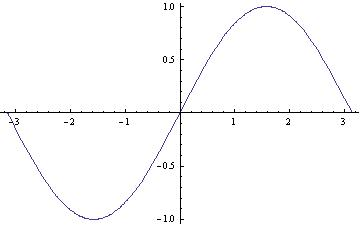
\includegraphics[height=2.5in, width=3.5in]{introduction/figures/sin_x.jpg}
\caption{Enjoyment and fun}
\end{figure}

Vestibulum ut urna eu turpis accumsan hendrerit. Mauris in mi sed eros auctor blandit. Nullam sit amet mauris vel eros aliquam pretium. Cras fermentum tortor. Sed egestas vulputate diam. Aenean sem dui, tincidunt a, ullamcorper eget, pharetra ac, tortor. In at sem vel elit bibendum convallis. Aenean ut enim vel leo malesuada dapibus. Etiam odio dolor, sollicitudin a, nonummy nec, tristique et, augue. Morbi ipsum. Aliquam venenatis. Proin orci. Duis sed quam eget turpis interdum feugiat.

\subsection{Hypothesis}  


Glossy prints of good reproducible quality, either black or white or color may be used. Photographs can be printed on 8 1/2$''$ x 11$''$ glossy finish paper, however, margin and page number requirements as stated above still apply for pages containing photographs. When attaching photographs to paper, double-sided tape may be used which causes the least amount of damage to the original paper.

The format of footnotes and the bibliography are to be prepared in accordance with standard practice in the field in which one is working. Documentation formatting style must be discussed with and accepted by the advisor. See further information on Reference Styles below.

The suggested typeface for dissertations is 10 to 12 point Arial. Other suggested fonts are Times New Roman and Helvetica. Script and italic fonts should not be used except as needed in the body of the paper. Consistency should be maintained throughout the paper, using the same font for all text, diagrams, etc. on all pages.

Electronic material, such as CDs and multimedia can accompany the dissertation. Each copy should be accompanied with a labeled CD. When bound, these are placed in an envelope in the back of the dissertation.  Oversized materials (pages greater than 8$''$ x 11$''$) can be included in the paper if necessary. Oversized pages should be folded so that 1$''$ on the left hand binding edge remains, allowing the page to be opened once the paper is bound.

The reference style used for formatting the paper must be confirmed with your department and advisor. Frequently used styles are the APA (American Psychological Association), MLA (Modern Language Association) and AMA (American Medical Association) styles. Style guides and manuals are available for each style. Page headers are not to be used.


\chapter{Methodology}
Three copies of the dissertation (1 original and 2 copies, either xerographic, photocopied, offset or letter quality printer) are to be supplied to the Library. In addition, an abstract independent of the document is to be supplied to the Library. The announcement for Ph.D. dissertation defense is to be given to The Office of the Registrar at least 1½ weeks prior to the defense. A sample defense announcement can be found in sample pages.

You must hand in your dissertation in person to the responsible person in the library. Dissertations cannot be mailed to the Library and cannot be handed in by another person.

\subsection*\normalsize\emph{Publication Agreement and Survey Forms}

The UMI Publication Agreement Form and a Survey of Earned Doctorates Form are submitted with the dissertation. The forms are available from Doris Oliver and online. Both forms must be completed and returned to Doris Oliver with the final dissertation. The UMI Publication Agreement Form includes the application form. This should be read, filled out and returned to Doris Oliver. The Survey of Earned Doctorates form is available online in two documents: the Survey of Earned Doctorates brochure and the Survey of Earned Doctorates form online.  UMI also provides a brochure on privacy as it relates to dissertations.

\subsection*\normalsize\emph{Use of Previously Published work in your dissertation}

If you are including previously published material as part of your dissertation, either as an appendix or as part of the body of your paper, you must obtain written permission from the publisher to have the work included as part of your paper.   Even if you are the author of the published material, you still must get permission from the publisher.    

Please view the dissertation specifications on the library website for information about UMI/Proquest's guide to copyright and copyright infringement. 

UMI/Proquest also includes information written by Kenneth Crews, a professor at Indiana University on the issue of copyright.  His work covers how to request permission from publishers, and sample permission letters.

\Large It is the responsibility of the student to ensure that all portions of their dissertation adhere to copyright law.  

\normalsize 


\chapter{Case Study}
All information about formatting a dissertation can be found on the library website at www.stevens.edu/library/services/phd.html.  Formatting information gets updated occasionally, so it is always good to check the requirements before submitting your dissertation.  

It is not required, but is strongly suggested that you make an appointment at the library to have the format of your dissertation reviewed before the final submission.  Dissertations can be rejected if they do not adhear to the formatting requirements.   

All information about formatting a dissertation can be found on the library website at www.stevens.edu/library/services/phd.html.  Formatting information gets updated occasionally, so it is always good to check the requirements before submitting your dissertation.  
It is not required, but is strongly suggested that you make an appointment at the library to have the format of your dissertation reviewed before the final submission.  Dissertations can be rejected if they do not adhear to the formatting requirements.   
All information about formatting a dissertation can be found on the library website at www.stevens.edu/library/services/phd.html.  Formatting information gets updated occasionally, so it is always good to check the requirements before submitting your dissertation.  

\begin{table}[htp]

\begin{center}
\begin{tabular}{|l|c|p{3.0in}|}
\hline
\multicolumn{3}{|c|}{Theoretical Dissertation Timeline}\\ \hline
Taskt&Time to Finish&Notes\\ \hline
Problem statement&10 hours&Initially very upbeat.\\ \hline
Research&3 days&Literature search to very previous studies.\\ \hline
Reformulation&4 hours&Presented and accepted by advisor\\ \hline
Research&20 days&Literature search to very previous  studies.\\ \hline
Experiments&14 days&Do some experiments and get results.\\ \hline
Format&1 day&Understand format guidelines for paper.\\ \hline
Write&years&Write the paper.\\ \hline
Revise&not too long&Proof read, etc.\\ \hline
Format&1-3 days&Verify correct report format is used.\\ \hline
See Library&1 hour&Meet with Doris to verify formatting.\\ \hline
Defend&1 day&Defend your research.\\ \hline
Revise&0 hours&It was perfect the first time.\\ \hline
Submit&1 day&Submit final dissertation to the library.\\ \hline
\end{tabular}
\end{center} 

\caption{Table of Tasks}\label{fig:erptsqfit}
\end{table}
It is not required, but is strongly suggested that you make an appointment at the library to have the format of your dissertation reviewed before the final submission.  Dissertations can be rejected if they do not adhear to the formatting requirements.   
All information about formatting a dissertation can be found on the library website at www.stevens.edu/library/services/phd.html.  Formatting information gets updated occasionally, so it is always good to check the requirements before submitting your dissertation.  
It is not required, but is strongly suggested that you make an appointment at the library to have the format of your dissertation reviewed before the final submission.  Dissertations can be rejected if they do not adhear to the formatting requirements.   
All information about formatting a dissertation can be found on the library website at www.stevens.edu/library/services/phd.html.  Formatting information gets updated occasionally, so it is always good to check the requirements before submitting your dissertation.  

It is not required, but is strongly suggested that you make an appointment at the library to have the format of your dissertation reviewed before the final submission.  Dissertations can be rejected if they do not adhear to the formatting requirements.   

\section{Further Analysis}  

\subsection*\normalsize\emph{Paper}
The original copy of the dissertation must be produced on good quality 8 1/2$''$ x 11$''$, 20 pound acid-free white paper. The paper should not be stapled, punched, bound, colored or printed on letterhead.

The two additional copies of the dissertation can be photocopied or produced on copier or laser paper.

\subsection*\normalsize\emph{Ink}
Black ink only is used to print your report.  If a graph or photograph contains color, that is fine. 

Latex is used to help in the printing of formulas.   The following formula would be difficult to reproduce in Microsoft Word: 
 \[
        \frac{d}{dx}\left( \int_{0}^{x} f(u)\,du\right)=f(x).
     \]

This Report was produced by LaTeX\footnote {\LaTeX\ is a fun typesetting program.} written by Barbara Arnett.  Barbara is not an expert with LaTeX, and anyone using LaTeX does not need to use this template.  It is simply provided to help with formatting, specifically with page numbers and images.  


%this subsection heading below will not show up in the table of contents.
\subsection*\normalsize\emph{Graphics} 

Graph paper may be used for original drawings, charts or illustrations. Original drawings may be in color or black and white, however, color is allowed for illustrations only; all text must appear in black. The original thesis must contain the original graphic or illustration, not a photocopy of the drawing, graphic or illustration.

If formulas and diagrams contain subscript and superscript characters, ensure they are large enough to read when printed in the final paper. 

\begin{figure}[htp]
\centering
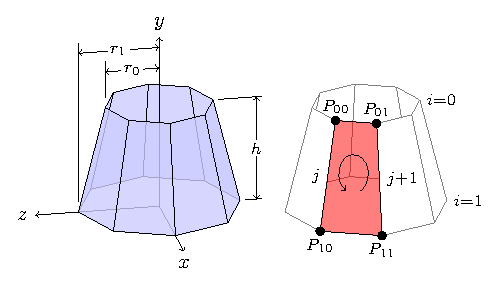
\includegraphics{casestudy/figures/3d-cone.pdf}
\caption{3D Cone}\label{fig:3d-cone}
\end{figure}

Photographs
Glossy prints of good reproducible quality, either black or white or color may be used. Photographs can be printed on 8 1/2$''$ x 11$''$ glossy finish paper, however, margin and page number requirements as stated above still apply for pages containing photographs. When attaching photographs to paper, double-sided tape may be used which causes the least amount of damage to the original paper. 

Graphics that are oriented in a landscape position must be done in a manner that retains the page numbering in the upper right hand corner, as shown in figure 3.2.  This can be difficult in Microsoft Word, but it is possible.  To do this in Microsoft Word, create a new section, change the page to landscape, and place the page number in a text box.  The text box then is rotated on the landscape page.    Then begin a new section and resume portrait orientation.

\begin{sidewaysfigure}
\centering
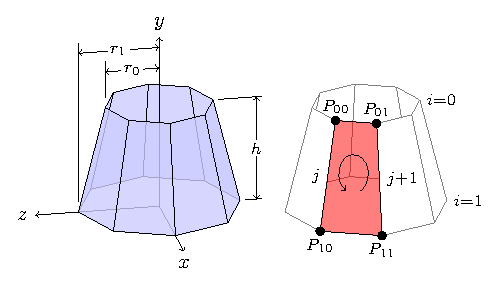
\includegraphics[height=5.0in, width=7.5in]{casestudy/figures/3d-cone.pdf}
\caption{This is an example of a landscape image within a page.  Note that the page number remains in the upper right hand corner of the page when the page is in the portrait position.}
\end{sidewaysfigure}

%!TEX root = ../thesis.tex
\chapter{Conclusions and Future Works}
\label{chap:chapter2}

\lipsum[2]

% At the end of each chapter
\newpage
%%%%% Appendices start %%%%%%%%%%%%%%%%
%% Comment out the following line if your thesis has no appendix
\addcontentsline{toc}{chapter}{Appendices}
\noindent \textbf{Appendices}
\appendix
\addcontentsline{toc}{section}{Appendix A}  %% removed \\
\noindent \textbf{Appendix A}
\vspace{12pt}

\noindent Appendices at the end of a dissertation are optional, and depend on the content of the dissertation. There can be one or more appendicies, however they should retain the page numbering requirements for dissertations.  Any concerns about the formatting of an appendix should be brought to Doris Oliver, who can direct you how to format your appendix if you have questions.

\begin{center}
\begin{tabular}{|l|c|p{3.0in}|}
\hline
\multicolumn{3}{|c|}{Theoretical Dissertation Timeline}\\ \hline
Taskt & Time to Finish & Notes\\ \hline
Problem statement & 10 hours & Initially very upbeat.\\ \hline
Research & 3 days&Literature search to very previous studies.\\ \hline
Reformulation&4 hours&Presented and accepted by advisor\\ \hline
Research&20 days&Literature search to very previous  studies.\\ \hline
Experiments&14 days&Do some experiments and get results.\\ \hline
Format&1 day&Understand format guidelines for paper.\\ \hline
Write&years&Write the paper.\\ \hline
Revise&not too long&Proof read, etc.\\ \hline
Format&1-3 days&Verify correct report format is used.\\ \hline
See Library&1 hour&Meet with Doris to verify formatting.\\ \hline
Defend&1 day&Defend your research.\\ \hline
Revise&0 hours&It was perfect the first time.\\ \hline
Submit&1 day&Submit final dissertation to the library.\\ \hline
\end{tabular}
\end{center}
\newpage

\addcontentsline{toc}{section}{Appendix B}  %% removed \\
\noindent \textbf{Appendix B}
\vspace{12pt}

\noindent Another one! Here is more text to go.
\newpage



%% Note: If your thesis has more than one appendix, NYU requires a "list of
%% appendices" page before the body of the thesis. I don't provide the tools
%% to create that here, so you're on your own for that one... Sorry.
%\addcontentsline{toc}{section}{Appendix B}  %% removed \\
\noindent \textbf{Appendix B}
\vspace{12pt}

\noindent Another one! Here is more text to go.
\newpage



%%%% Input bibliography file %%%%%%%%%%%%%%%
% %% Modified by Abdullah Khanfor for Stevens Institute of Technology PhD thesis format design guidelines 2019-2020
% NYU PhD thesis format. Original template created by José Koiller 2007--2008.
%% Updated by Anshul Vikram Pandey with new design guidelines. 2017-2018

%% Use the first of the following lines during production to
%% easily spot "overfull boxes" in the output. Use the second
%% line for the final version.
% \documentclass[12pt,draft,letterpaper]{report}
% \documentclass[12pt,letterpaper]{report}
\documentclass[12pt]{report}

%% Replace the title, name, advisor name, graduation date and dedication below with
%% your own. Graduation months must be January, May or September.
\newcommand{\thesistitle}{TITLE TO JUSTIFY YOUR PHD YEARS}
\newcommand{\thesisauthor}{Your Name}
\newcommand{\thesisadvisor}{Your Advisor's Name}
\newcommand{\thesisyear}{2020}
\newcommand{\thesisname}{Abdullah Khanfor}
\newcommand{\thesischairadvisor}{Dr. }    % this name prints on the title page as chairman and the abstract page as advisor
\newcommand{\committeenameA}{Dr. }
\newcommand{\committeenameB}{Dr. }
\newcommand{\committeenameC}{Dr. }
\newcommand{\thesisdepartment}{Systems Engineering}
\newcommand{\thesisdate}{November 22, 2020}
\newcommand{\thesistype}{dissertation}
\newcommand{\thesisdegree}{Doctor of Philosophy}
\newcommand{\graddate}{\the\year} % like 2020, 2019, no month or day should be written
\newcommand{\thesissigline}[1]{%
  \leftline{\hbox to 2.5in{}\hrulefill}
  \endgraf
  \vspace*{-18pt}
  \leftline{\hbox to 2.53in{}{#1}}}

%% If you do not want a dedication, scroll down and comment out
%% the appropriate lines in this file.
\newcommand{\thesisdedication}{To all the Ph.D. pursuing brave souls}

%% The following makes chapters and sections, but not subsections,
%% appear in the TOC (table of contents). Increase to 2 or 3 to
%% make subsections or subsubsections appear, respectively. It seems
%% to be usual to use the "1" setting, however.
\setcounter{tocdepth}{1}

%% Sectional units up to subsubsections are numbered. To number
%% subsections, but not subsubsections, decrease this counter to 2.
\setcounter{secnumdepth}{3}

% Setting a gap between page number and text block

%% This inputs your auxiliary file with \usepackage's and \newcommand's:
%% It is assumed that that file is called "definitions.tex".
%%
%% Place here your \usepackage's. Some recommended packages are already included.
%%

% Graphics:
\usepackage[final]{graphicx}
%\usepackage{graphicx} % use this line instead of the above to suppress graphics in draft copies
%\usepackage{graphpap} % \defines the \graphpaper command

% Indent first line of each section:
%\usepackage{indentfirst}

% Good AMS stuff:
\usepackage{amsthm} % facilities for theorem-like environments
\usepackage[tbtags]{amsmath} % a lot of good stuff!

% Fonts and symbols:
\usepackage{amsfonts}
\usepackage{amssymb}

\usepackage{xspace}
\usepackage{algorithmic}
\usepackage{algorithm}
\usepackage{microtype}
\usepackage{subfigure}
\usepackage{color}
\usepackage{todonotes}
\usepackage{url}
\newfloat{algorithm}{t}{lop}

\usepackage{blindtext}

%% Controls spacing between lines (\doublespacing, \onehalfspacing, etc.):
\usepackage[utf8x]{inputenc}
\usepackage{fancyhdr}

% This package to change the font if the document. This font is optional as you preference. You can comment it to use the CMU font
%\usepackage{helvet}
%\renewcommand{\familydefault}{\sfdefault}

%% \usepackage{amsmath}
%% \usepackage{amssymb}
\usepackage{lipsum}
% \newfloat{algorithm}{t}{lop}

% Packages for setting the length and width of document
\usepackage{setspace}

% Package for sideway images and figures
\usepackage{rotating}
\usepackage{pdflscape}

% Formatting tools:
%\usepackage{relsize} % relative font size selection, provides commands \textsmalle, \textlarger
%\usepackage{xspace} % gentle spacing in macros, such as \newcommand{\acims}{\textsc{acim}s\xspace}

% Page formatting utility:
%\usepackage{geometry}
\usepackage{multirow}

\usepackage{listings}

% For citations
\usepackage[numbers,sort]{natbib}
\usepackage[nottoc]{tocbibind}

\usepackage[all,cmtip]{xy}

% Change the color of the hyperlinks and titles from blue to black
\usepackage{hyperref}
\hypersetup{
    colorlinks = false,
    linkbordercolor = {white},
    linkcolor=black,
    filecolor=black,
    urlcolor=black,
    citecolor=black
}

%%
%% Place here your \newcommand's and \renewcommand's. Some examples already included.
%%
%\newcommand{\acims}{\textsc{acim}s\xspace}
\newcommand{\Mspace}        {{\mathbb M}}
\newcommand{\Rspace}        {{\mathbb R}}
\newcommand{\Cspace}        {{\mathbb C}}

\newcommand{\Mo}        {{\hat M}}
\newcommand{\Ms}        {{\tilde M}}
\newcommand{\Do}          {{\hat D}}
\newcommand{\Ds}        {{\tilde D}}
\newcommand{\doo}          {{\hat d}}
\newcommand{\dss}        {{\tilde d}}
\newcommand{\w}        {{\mathbf w}}

% general
\newcommand{\ie}{i.e.}
\newcommand{\eg}{e.g.}
\newcommand{\reffig}[1]{{Figure~\ref{#1}}}
\newcommand{\refchap}[1]{{Chapter~\ref{#1}}}
\newcommand{\refsec}[1]{{Section~\ref{#1}}}
\newcommand{\reftab}[1]{{Table~\ref{#1}}}
\newcommand{\refapp}[1]{{Appendix~\ref{#1}}}
\newcommand{\refeq}[1]{{Equation~\ref{#1}}}
\newcommand{\refalg}[1]{{Algorithm~\ref{#1}}}
\newcommand{\myparagraph}[1]{\noindent \textbf{#1}}
\newcommand{\highlight}[1]{{\color{black}#1}}

%%
%% Place here your \newtheorem's:
%%

%% Some examples commented out below. Create your own or use these...
%%%%%%%%%\swapnumbers % this makes the numbers appear before the statement name.
%\theoremstyle{plain}
%\newtheorem{thm}{Theorem}[chapter]
%\newtheorem{prop}[thm]{Proposition}
%\newtheorem{lemma}[thm]{Lemma}
%\newtheorem{cor}[thm]{Corollary}

%\theoremstyle{definition}
%\newtheorem{define}{Definition}[chapter]

%\theoremstyle{remark}
%\newtheorem*{rmk*}{Remark}
%\newtheorem*{rmks*}{Remarks}

%% This defines the "proo" environment, which is the same as proof, but
%% with "Proof:" instead of "Proof.". I prefer the former.
%\newenvironment{proo}{\begin{proof}[Proof:]}{\end{proof}}

%\usepackage[subfigure]{tocloft}
\usepackage[explicit]{titlesec}%
\usepackage{titletoc}
\usepackage{etoolbox}

% To add space between the Table of Contents, List of Figures and the List of Tables and the list content
\addtocontents{toc}{\vspace{1.2cm}}
\addtocontents{lof}{\vspace{1.2cm}}
\addtocontents{lot}{\vspace{1.2cm}}

% This command for chapters
\newcommand\chap[1]{%
  \chapter*{#1}%
  \addcontentsline{toc}{chapter}{#1}}

% Table of contents formatting
% Removing the dots between the Title and the page number
\makeatletter
\renewcommand{\@dotsep}{10000} 
\makeatother

\usepackage{tabto}
\usepackage{makebox}

% Table of contents font and space modifications

\titlecontents{chapter}[0pt]
    {\vskip 10pt \bfseries}
    {\bfseries\text{Chapter }\thecontentslabel\tabto{3.5cm}}
    {}
    {\hfill\bfseries\contentspage}

\titlecontents{section}[0pt]
    {}
    {\quad\quad\thecontentslabel\tabto{3.5cm}}
    {}
    {\hfill\contentspage}

\titlecontents{subsection}[0pt]
    {}
    {\quad\quad\thecontentslabel\tabto{3.5cm}}
    {}
    {\hfill\contentspage}
    
\titlecontents{table}[0pt]
    {}
    {\quad\quad\thecontentslabel\tabto{3.5cm}}
    {}
    {\hfill\contentspage}

\titlecontents{figure}[0pt]
    {}
    {\quad\quad\thecontentslabel\tabto{3.5cm}}
    {}
    {\hfill\contentspage}

% Change the Table of Contents, List of Tables ... etc. font size insited of big font
\renewcommand{\contentsname}{\normalsize{Table of Contents}}
\renewcommand{\listfigurename}{\normalsize{List of Figures}}
\renewcommand{\listtablename}{\normalsize{List of Tables}}
\renewcommand{\bibname}{\normalsize{Bibliography}}
\renewcommand{\indexname}{\normalsize{Index}}

% May 2009 added this to move page number up a bit
\addtolength{\voffset}{-2em}

% This is to format the chapter tags in this file
\usepackage{chngcntr}
\usepackage{lipsum}% just to generate text for the example

%% Page layout (customized to letter paper and Stevens requirements):
% if not using pdflatex to produce output, you may need to change to pagewidth and pageheight variables.
%\pagewidth 8.5in
%\pageheight 11in 
\pdfpagewidth 8.5in
\pdfpageheight 11in 
%
\setlength{\textheight}{8.5in} 
\setlength{\oddsidemargin}{0.5in}  
\setlength{\evensidemargin}{0.5in} 
\setlength{\textwidth}{6.0in}
\setlength{\topmargin}{0.in}    
\setlength{\headheight}{0.5in}
\setlength{\headwidth}{6.0in}
% change from .25in to .5 in May 2009 
\setlength{\headsep}{0.65in}
\setlength{\parindent}{12mm}

% For each chapter and section titles in the rest of the document the font formatting

% Chapter styles
\usepackage{sectsty}

\chapternumberfont{\normalsize} 
\chaptertitlefont{\normalsize}

\makeatletter
% No extra space between chapter number and chapter header lines:
\patchcmd{\@makechapterhead} {\vskip 20}{\vskip 0} {}{}
% Reduce extra space between chapter header and section header lines by 50%:
\patchcmd{\@makechapterhead} {\vskip 40}{\vskip 20}{}{}
\patchcmd{\@makeschapterhead}{\vskip 40}{\vskip 20}{}{} % for unnumbered chapters
\makeatother

% Sections styles
\sectionfont{\normalsize}

% Sub-sections styles
\subsectionfont{\normalsize}



%% Use the following commands, if desired, during production.
%% Comment them out for final version.
%\usepackage{layout} % defines the \layout command, see below
%\setlength{\hoffset}{-.75in} % creates a large right margin for notes and \showlabels

\pagestyle{fancy}
\fancyhf{}
% this prints a line under the header
\renewcommand{\headrulewidth}{0 pt}
%this prints a line under the footer
\renewcommand{\footrulewidth}{0 pt}
\fancyhead[RO]{}
\fancyhead[LO]{}
\fancyfoot[C]{}
\rhead{\thepage}

\fancypagestyle{plain}{%
\fancyhf{}
\rhead{\thepage}
}

%% Page layout (customized to letter paper and NYU requirements):
\setlength{\headheight}{20pt} 

%% Use the line below for official NYU version, which requires
%% double line spacing. For all other uses, this is unnecessary,
%% so the line can be commented out.
\onehalfspacing % requires package setspace, invoked above

%% Each of the following lines defines the \com command, which produces
%% a comment (notes for yourself, for instance) in the output file.
%% Example:    \com{this will appear as a comment in the output}
%% Choose (uncomment) only one of the three forms:
%\newcommand{\com}[1]{[/// {#1} ///]}       % between [/// and ///].
\newcommand{\com}[1]{\marginpar{\tiny #1}} % as (tiny) margin notes
%\newcommand{\com}[1]{}                     % suppress all comments.

%% Cross-referencing utilities. Use one or the other--whichever you prefer--
%% but comment out both lines for final version.
%\usepackage{showlabels}
%\usepackage{showkeys}
% \pagestyle{headings}

\begin{document}
%% Produces a test "layout" page, for "debugging" purposes only.
%% Comment out for final version.
%\layout % requires package layout (see above, on this same file)
%% Sets page numbering to "roman style" i, ii, iii, iv, etc:

%%%%%% Cover page %%%%%%%%%%%
%% Sets page numbering to "roman style" i, ii, iii, iv, etc:
\pagenumbering{roman}
\thispagestyle{empty}
\begin{center}
{
  {\thesistitle}
  \vspace{.15in}
  
    by
    
  \vspace{.15in}
  \thesisauthor
  
  \vspace{.15in}
  
 {A DISSERTATION}\\
  \vspace{.2in}
  \begin{spacing}{1}
    {Submitted to the Faculty of the Stevens Institute of Technology\\
    in partial fulfillment of the requirements for the degree of}
    \end{spacing}
  \vspace{.2in}
  
  {DOCTOR OF PHILOSOPHY}\\
  \vspace{1.0in}
  % for master thesis, change Chairman to Advisor
    \hfill 
    \begin{minipage}{80mm}
    \begin{spacing}{ }\noindent \rule{3.2in}{0.1mm}
        \thesisname, Candidate\\[3mm]
        \underline{ADVISORY COMMITTEE}\\[3mm]
        \noindent \rule{3.2in}{0.1mm}\\[-1.3mm]
        % for master thesis, change Chairman to Advisor
        {\thesischairadvisor}, Chairman  \hfill{Date}\\[2mm]
        {\noindent \rule{3.2in}{0.1mm}}\\[-1.3mm]
        {\committeenameA}        \hfill{Date}\\[2mm]
        {\noindent \rule{3.2in}{0.1mm}}\\[-1.3mm]
        {\committeenameB}        \hfill{Date}\\[2mm]
        {\noindent \rule{3.2in}{0.1mm}}\\[-1.3mm]
        {\committeenameC}        \hfill{Date}\\[2mm]
    \end{spacing}
  \end{minipage}
  \vfill
  
  {STEVENS INSTITUTE OF TECHNOLOGY\\
  \vspace{-0.05in}
  Castle Point on Hudson\\
  Hoboken, NJ 07030
  }
  % \vfill

  {\graddate}
}

\end{center}

\newpage



%%%%%%%%%%%%%% Microfilm / Publishing Page ProQuest %%%%%%%%%%%%%%%%%
% You can comment this section it is here to show you how it will appear when it submitted.
\thispagestyle{empty}
\begin{center}
ProQuest Number: XXXXXXXX

\vspace{.45in}

All rights reserved.

\vspace{.1in}

INFORMATION TO ALL USERS\\
The quality of this reproduction is dependent upon the quality of the copy submitted.
\vspace{.2in}

In the unlikely event hat  the author did not send a complete manuscript and there are missing pages, these will be  noted. Also ,if material had to be removed, a note will indicate the deletion.

\vspace{.1in}

\begin{figure}[H]
  \centering
  \includegraphics[width=200px]{misc/proquest-seeklogo.eps}
\end{figure}

\vspace{.1in}

ProQuest Number: XXXXXXXX

\vspace{.1in}

Published  by  ProQuest  LLC (\the\year).        Copyright of the Dissertation is held by the Author.

\vspace{.2in}

All rights reserved. This work is protected against  unauthorized copying under Title 17, United States Code Microform Edition {\textcopyright} ProQuest  LLC.

\vspace{.2in}

ProQuest LLC.\\
789 East Eisenhower Parkway\\
P.O. Box 1346\\
Ann Arbor, MI  48106-1346

\end{center}
\newpage

%%%%%% Copyrights page %%%%%%%%%%%
%
\setcounter{page}{2}
%% No numbering in the title page:
\thispagestyle{empty}
%
\begin{center}
{
  \vspace*{\fill}

  {\textcopyright} \graddate, \thesisname. All rights reserved.
}

\end{center}

\newpage
\doublespacing

%%%%%%%%%%%%%% Abstract %%%%%%%%%%%%%%%%%
\begin{center}
    {\thesistitle}\\ 
    {ABSTRACT}\\
    \vspace{.05in}
\end{center}
\addcontentsline{toc}{chapter}{Abstract}
%!TEX root = thesis.tex

%
An abstract of 350 words or less, not including the title, is required for all dissertations and theses. One extra, loose copy of your abstract is required for the library. In addition, an abstract is required as part of the PhD.  If your abstract is longer than 350 words, UMI (the publisher of dissertations) might edit your abstract to 350 words. It is in your best interest to do the editing yourself.  

The abstract should be formatted as it is shown here.  The requirements are as follows:   Title of document on top;  Abstract of document (350 words or fewer); Author's name on bottom; Advisor's name on bottom; Date on bottom; Department at bottom; Degree on bottom; The abstract should be the first page where page numbers appear, starting with page number iii (or page ii if a copyright page is not included). All pages after the abstract up to the first page of the body of the document continue with lower case Roman numerals (iii, iv, v, etc.)

Note: 1 extra, loose copy of your abstract is required for the Library. In addition, an abstract is required as part of the Ph.D defense announcement to be submitted to the Office of the Registrar at least 1½ weeks prior to the scheduled date of defense. 


\vspace{0.4in}
\begin{flushleft}
Author: \thesisname \\
Advisor: \thesischairadvisor \\
Date: \thesisdate \\
Department: \thesisdepartment \\
Degree: \thesisdegree \\
\end{flushleft}
\newpage

%%%%%%%%%%%%%% Dedication Page %%%%%%%%%%%%%%%%%
%% Comment out the following lines if you do not want to dedicate it is optional
\chapter*{Dedication}
\addcontentsline{toc}{chapter}{Dedication}
\strut \vspace{2in}
\begin{center}
``Most people are other people. Their thoughts are someone else's opinions, their lives a mimicry, their passions a quotation."
    \end{center}
    \vfill \strut
    \newpage
\newpage

%%%%%%%%%%%%%% Acknowledgements %%%%%%%%%%%%%%%%%
%% Comment out the following lines if you do not want to acknowledge
%% anyone's help...
\addcontentsline{toc}{chapter}{Acknowledgements}
%!TEX root = thesis.tex

%% Write your acknowledgements in this file. If you do not want to acknowledge anyone,
%% you can delete this file and comment out the corresponding part in the "thesis.tex"
%% file.
\noindent \textbf{Acknowledgments} \\[6mm]
\blindtext
    \vfill \strut


\newpage

%%%% Table of Contents %%%%%%%%%%%%
\setcounter{tocdepth}{3} % To show a three level depth of sections

\tableofcontents

% \clearpage
% \pagestyle{headings}
\newpage

%%%%% List of Tables %%%%%%%%%%%%%
%% Comment out the following two lines if your thesis does not
%% contain any tables. The list of tables contains only
%% those tables included withing the "table" environment.
\listoftables\addcontentsline{toc}{chapter}{\listtablename}
\newpage

%%%%% List of Figures %%%%%%%%%%%%%
%% Comment out the following two lines if your thesis does not
%% contain any figures. The list of figures contains only
%% those figures included withing the "figure" environment.
\listoffigures\addcontentsline{toc}{chapter}{\listfigurename}
\newpage

%%%%% Body of thesis starts %%%%%%%%%%%%
\pagenumbering{arabic} % switches page numbering to arabic: 1, 2, 3, etc.

%% Introduction. If your thesis has no introduction, or chapter 1 is
%% meant to be the introduction, then comment out the lines below.
%% \section*{Introduction}\addcontentsline{toc}{section}{Introduction}
%\input{intro}

%%If your thesis has different "Parts", use commands such as the following:


\chapter{Introduction}
This sample dissertation is provided for help is viewing the layout of a dissertation.  The content is not at all anything that one would put in a dissertation.  To view previous dissertations submitted by Stevens students, please go to the online resources section of the library website, and go to the database Stevens Dissertations Online.  

\section{The Problem Statement}    
Page numbers in a dissertation must be formatted as they are in this document.  

Arabic numerals (1, 2, 3...) must appear in the upper right-hand corner of every page starting with the first page of the body of the paper (usually the introduction or the first page of the first chapter). If it is necessary to print some pages in landscape format or if oversize pages or materials are necessary, adjust formatting so that the page number on these pages will appear in the upper right-hand corner of the page when the document is bound. Page numbers appear on every page of the body of the document, including the bibliography and the vita.

Lower case Roman numerals (i, ii, iii...) must be used for the pages appearing before the body of the paper (called the front matter). The title page is considered page i, but there is no page number printed on the title page. The copyright page (if it is included) is considered page ii, but there is no page number printed on the copyright page. The remainder of the front matter (abstract, table of contents, etc.) is numbered with lowercase Roman numerals, starting with page iii (if no copyright page is used, the first page of the front matter is printed with page number ii). 

There is no required citation style for references or a bibliography in a dissertation.  If your advisor or department has a required or suggested citation style, that should be what is used in the dissertation.  Frequently used citation styles are MLA\cite{gibaldi_mla}, APA style\cite{APA}, Chicago, ASM and AIP.    

\section{Problem Scope}
Page numbers in a dissertation must be formatted as they are in this document.  

Arabic numerals (1, 2, 3...) must appear in the upper right-hand corner of every page starting with the first page of the body of the paper (usually the introduction or the first page of the first chapter). If it is necessary to print some pages in landscape format or if oversize pages or materials are necessary, adjust formatting so that the page number on these pages will appear in the upper right-hand corner of the page when the document is bound. Page numbers appear on every page of the body of the document, including the bibliography and the vita.

Lower case Roman numerals (i, ii, iii...) must be used for the pages appearing before the body of the paper (called the front matter). The title page is considered page i, but there is no page number printed on the title page. The copyright page (if it is included) is considered page ii, but there is no page number printed on the copyright page. The remainder of the front matter (abstract, table of contents, etc.) is numbered with lowercase Roman numerals, starting with page iii (if no copyright page is used, the first page of the front matter is printed with page number ii). 

There is no required citation style for references or a bibliography in a dissertation \cite{rabinowitz_manual_2009}.  If your advisor or department has a required or suggested citation style, that should be what is used in the dissertation.  Frequently used citation styles are MLA \cite{gibaldi_mla}, APA style \cite{APA}, Chicago, ASM and AIP.    

If we allow x to go to infinity, you see that 
$\sum_{i=1}^{\infty} x_{i}$.  As follows, $\sqrt{x+y}$ proves the theorem to be correct.
 
\section{Research Approach}
Good research is essential is producing a dissertation or thesis.  The reference librarians at stevens are always available to help you navigate the world of online research.  Feel free to make an appointment, or watch for one of the workshops given about doing your research for your dissertation.  

\begin{figure}
\centering
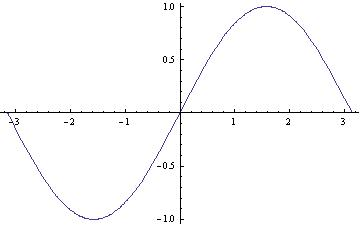
\includegraphics[height=2.5in, width=3.5in]{introduction/figures/sin_x.jpg}
\caption{Enjoyment and fun}
\end{figure}

Vestibulum ut urna eu turpis accumsan hendrerit. Mauris in mi sed eros auctor blandit. Nullam sit amet mauris vel eros aliquam pretium. Cras fermentum tortor. Sed egestas vulputate diam. Aenean sem dui, tincidunt a, ullamcorper eget, pharetra ac, tortor. In at sem vel elit bibendum convallis. Aenean ut enim vel leo malesuada dapibus. Etiam odio dolor, sollicitudin a, nonummy nec, tristique et, augue. Morbi ipsum. Aliquam venenatis. Proin orci. Duis sed quam eget turpis interdum feugiat.

\subsection{Hypothesis}  


Glossy prints of good reproducible quality, either black or white or color may be used. Photographs can be printed on 8 1/2$''$ x 11$''$ glossy finish paper, however, margin and page number requirements as stated above still apply for pages containing photographs. When attaching photographs to paper, double-sided tape may be used which causes the least amount of damage to the original paper.

The format of footnotes and the bibliography are to be prepared in accordance with standard practice in the field in which one is working. Documentation formatting style must be discussed with and accepted by the advisor. See further information on Reference Styles below.

The suggested typeface for dissertations is 10 to 12 point Arial. Other suggested fonts are Times New Roman and Helvetica. Script and italic fonts should not be used except as needed in the body of the paper. Consistency should be maintained throughout the paper, using the same font for all text, diagrams, etc. on all pages.

Electronic material, such as CDs and multimedia can accompany the dissertation. Each copy should be accompanied with a labeled CD. When bound, these are placed in an envelope in the back of the dissertation.  Oversized materials (pages greater than 8$''$ x 11$''$) can be included in the paper if necessary. Oversized pages should be folded so that 1$''$ on the left hand binding edge remains, allowing the page to be opened once the paper is bound.

The reference style used for formatting the paper must be confirmed with your department and advisor. Frequently used styles are the APA (American Psychological Association), MLA (Modern Language Association) and AMA (American Medical Association) styles. Style guides and manuals are available for each style. Page headers are not to be used.


\chapter{Methodology}
Three copies of the dissertation (1 original and 2 copies, either xerographic, photocopied, offset or letter quality printer) are to be supplied to the Library. In addition, an abstract independent of the document is to be supplied to the Library. The announcement for Ph.D. dissertation defense is to be given to The Office of the Registrar at least 1½ weeks prior to the defense. A sample defense announcement can be found in sample pages.

You must hand in your dissertation in person to the responsible person in the library. Dissertations cannot be mailed to the Library and cannot be handed in by another person.

\subsection*\normalsize\emph{Publication Agreement and Survey Forms}

The UMI Publication Agreement Form and a Survey of Earned Doctorates Form are submitted with the dissertation. The forms are available from Doris Oliver and online. Both forms must be completed and returned to Doris Oliver with the final dissertation. The UMI Publication Agreement Form includes the application form. This should be read, filled out and returned to Doris Oliver. The Survey of Earned Doctorates form is available online in two documents: the Survey of Earned Doctorates brochure and the Survey of Earned Doctorates form online.  UMI also provides a brochure on privacy as it relates to dissertations.

\subsection*\normalsize\emph{Use of Previously Published work in your dissertation}

If you are including previously published material as part of your dissertation, either as an appendix or as part of the body of your paper, you must obtain written permission from the publisher to have the work included as part of your paper.   Even if you are the author of the published material, you still must get permission from the publisher.    

Please view the dissertation specifications on the library website for information about UMI/Proquest's guide to copyright and copyright infringement. 

UMI/Proquest also includes information written by Kenneth Crews, a professor at Indiana University on the issue of copyright.  His work covers how to request permission from publishers, and sample permission letters.

\Large It is the responsibility of the student to ensure that all portions of their dissertation adhere to copyright law.  

\normalsize 


\chapter{Case Study}
All information about formatting a dissertation can be found on the library website at www.stevens.edu/library/services/phd.html.  Formatting information gets updated occasionally, so it is always good to check the requirements before submitting your dissertation.  

It is not required, but is strongly suggested that you make an appointment at the library to have the format of your dissertation reviewed before the final submission.  Dissertations can be rejected if they do not adhear to the formatting requirements.   

All information about formatting a dissertation can be found on the library website at www.stevens.edu/library/services/phd.html.  Formatting information gets updated occasionally, so it is always good to check the requirements before submitting your dissertation.  
It is not required, but is strongly suggested that you make an appointment at the library to have the format of your dissertation reviewed before the final submission.  Dissertations can be rejected if they do not adhear to the formatting requirements.   
All information about formatting a dissertation can be found on the library website at www.stevens.edu/library/services/phd.html.  Formatting information gets updated occasionally, so it is always good to check the requirements before submitting your dissertation.  

\begin{table}[htp]

\begin{center}
\begin{tabular}{|l|c|p{3.0in}|}
\hline
\multicolumn{3}{|c|}{Theoretical Dissertation Timeline}\\ \hline
Taskt&Time to Finish&Notes\\ \hline
Problem statement&10 hours&Initially very upbeat.\\ \hline
Research&3 days&Literature search to very previous studies.\\ \hline
Reformulation&4 hours&Presented and accepted by advisor\\ \hline
Research&20 days&Literature search to very previous  studies.\\ \hline
Experiments&14 days&Do some experiments and get results.\\ \hline
Format&1 day&Understand format guidelines for paper.\\ \hline
Write&years&Write the paper.\\ \hline
Revise&not too long&Proof read, etc.\\ \hline
Format&1-3 days&Verify correct report format is used.\\ \hline
See Library&1 hour&Meet with Doris to verify formatting.\\ \hline
Defend&1 day&Defend your research.\\ \hline
Revise&0 hours&It was perfect the first time.\\ \hline
Submit&1 day&Submit final dissertation to the library.\\ \hline
\end{tabular}
\end{center} 

\caption{Table of Tasks}\label{fig:erptsqfit}
\end{table}
It is not required, but is strongly suggested that you make an appointment at the library to have the format of your dissertation reviewed before the final submission.  Dissertations can be rejected if they do not adhear to the formatting requirements.   
All information about formatting a dissertation can be found on the library website at www.stevens.edu/library/services/phd.html.  Formatting information gets updated occasionally, so it is always good to check the requirements before submitting your dissertation.  
It is not required, but is strongly suggested that you make an appointment at the library to have the format of your dissertation reviewed before the final submission.  Dissertations can be rejected if they do not adhear to the formatting requirements.   
All information about formatting a dissertation can be found on the library website at www.stevens.edu/library/services/phd.html.  Formatting information gets updated occasionally, so it is always good to check the requirements before submitting your dissertation.  

It is not required, but is strongly suggested that you make an appointment at the library to have the format of your dissertation reviewed before the final submission.  Dissertations can be rejected if they do not adhear to the formatting requirements.   

\section{Further Analysis}  

\subsection*\normalsize\emph{Paper}
The original copy of the dissertation must be produced on good quality 8 1/2$''$ x 11$''$, 20 pound acid-free white paper. The paper should not be stapled, punched, bound, colored or printed on letterhead.

The two additional copies of the dissertation can be photocopied or produced on copier or laser paper.

\subsection*\normalsize\emph{Ink}
Black ink only is used to print your report.  If a graph or photograph contains color, that is fine. 

Latex is used to help in the printing of formulas.   The following formula would be difficult to reproduce in Microsoft Word: 
 \[
        \frac{d}{dx}\left( \int_{0}^{x} f(u)\,du\right)=f(x).
     \]

This Report was produced by LaTeX\footnote {\LaTeX\ is a fun typesetting program.} written by Barbara Arnett.  Barbara is not an expert with LaTeX, and anyone using LaTeX does not need to use this template.  It is simply provided to help with formatting, specifically with page numbers and images.  


%this subsection heading below will not show up in the table of contents.
\subsection*\normalsize\emph{Graphics} 

Graph paper may be used for original drawings, charts or illustrations. Original drawings may be in color or black and white, however, color is allowed for illustrations only; all text must appear in black. The original thesis must contain the original graphic or illustration, not a photocopy of the drawing, graphic or illustration.

If formulas and diagrams contain subscript and superscript characters, ensure they are large enough to read when printed in the final paper. 

\begin{figure}[htp]
\centering
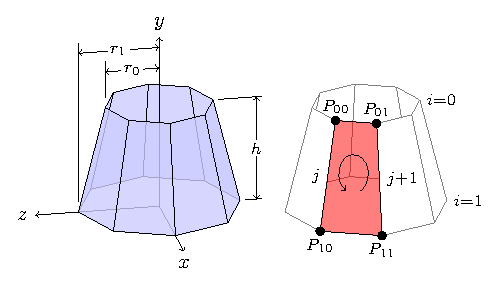
\includegraphics{casestudy/figures/3d-cone.pdf}
\caption{3D Cone}\label{fig:3d-cone}
\end{figure}

Photographs
Glossy prints of good reproducible quality, either black or white or color may be used. Photographs can be printed on 8 1/2$''$ x 11$''$ glossy finish paper, however, margin and page number requirements as stated above still apply for pages containing photographs. When attaching photographs to paper, double-sided tape may be used which causes the least amount of damage to the original paper. 

Graphics that are oriented in a landscape position must be done in a manner that retains the page numbering in the upper right hand corner, as shown in figure 3.2.  This can be difficult in Microsoft Word, but it is possible.  To do this in Microsoft Word, create a new section, change the page to landscape, and place the page number in a text box.  The text box then is rotated on the landscape page.    Then begin a new section and resume portrait orientation.

\begin{sidewaysfigure}
\centering
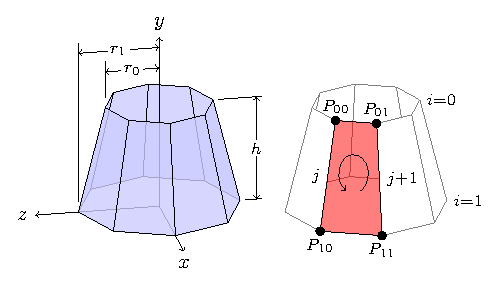
\includegraphics[height=5.0in, width=7.5in]{casestudy/figures/3d-cone.pdf}
\caption{This is an example of a landscape image within a page.  Note that the page number remains in the upper right hand corner of the page when the page is in the portrait position.}
\end{sidewaysfigure}

%!TEX root = ../thesis.tex
\chapter{Conclusions and Future Works}
\label{chap:chapter2}

\lipsum[2]

% At the end of each chapter
\newpage
%%%%% Appendices start %%%%%%%%%%%%%%%%
%% Comment out the following line if your thesis has no appendix
\addcontentsline{toc}{chapter}{Appendices}
\noindent \textbf{Appendices}
\appendix
\addcontentsline{toc}{section}{Appendix A}  %% removed \\
\noindent \textbf{Appendix A}
\vspace{12pt}

\noindent Appendices at the end of a dissertation are optional, and depend on the content of the dissertation. There can be one or more appendicies, however they should retain the page numbering requirements for dissertations.  Any concerns about the formatting of an appendix should be brought to Doris Oliver, who can direct you how to format your appendix if you have questions.

\begin{center}
\begin{tabular}{|l|c|p{3.0in}|}
\hline
\multicolumn{3}{|c|}{Theoretical Dissertation Timeline}\\ \hline
Taskt & Time to Finish & Notes\\ \hline
Problem statement & 10 hours & Initially very upbeat.\\ \hline
Research & 3 days&Literature search to very previous studies.\\ \hline
Reformulation&4 hours&Presented and accepted by advisor\\ \hline
Research&20 days&Literature search to very previous  studies.\\ \hline
Experiments&14 days&Do some experiments and get results.\\ \hline
Format&1 day&Understand format guidelines for paper.\\ \hline
Write&years&Write the paper.\\ \hline
Revise&not too long&Proof read, etc.\\ \hline
Format&1-3 days&Verify correct report format is used.\\ \hline
See Library&1 hour&Meet with Doris to verify formatting.\\ \hline
Defend&1 day&Defend your research.\\ \hline
Revise&0 hours&It was perfect the first time.\\ \hline
Submit&1 day&Submit final dissertation to the library.\\ \hline
\end{tabular}
\end{center}
\newpage

\addcontentsline{toc}{section}{Appendix B}  %% removed \\
\noindent \textbf{Appendix B}
\vspace{12pt}

\noindent Another one! Here is more text to go.
\newpage



%% Note: If your thesis has more than one appendix, NYU requires a "list of
%% appendices" page before the body of the thesis. I don't provide the tools
%% to create that here, so you're on your own for that one... Sorry.
%\addcontentsline{toc}{section}{Appendix B}  %% removed \\
\noindent \textbf{Appendix B}
\vspace{12pt}

\noindent Another one! Here is more text to go.
\newpage



%%%% Input bibliography file %%%%%%%%%%%%%%%
% %% Modified by Abdullah Khanfor for Stevens Institute of Technology PhD thesis format design guidelines 2019-2020
% NYU PhD thesis format. Original template created by José Koiller 2007--2008.
%% Updated by Anshul Vikram Pandey with new design guidelines. 2017-2018

%% Use the first of the following lines during production to
%% easily spot "overfull boxes" in the output. Use the second
%% line for the final version.
% \documentclass[12pt,draft,letterpaper]{report}
% \documentclass[12pt,letterpaper]{report}
\documentclass[12pt]{report}

%% Replace the title, name, advisor name, graduation date and dedication below with
%% your own. Graduation months must be January, May or September.
\newcommand{\thesistitle}{TITLE TO JUSTIFY YOUR PHD YEARS}
\newcommand{\thesisauthor}{Your Name}
\newcommand{\thesisadvisor}{Your Advisor's Name}
\newcommand{\thesisyear}{2020}
\newcommand{\thesisname}{Abdullah Khanfor}
\newcommand{\thesischairadvisor}{Dr. }    % this name prints on the title page as chairman and the abstract page as advisor
\newcommand{\committeenameA}{Dr. }
\newcommand{\committeenameB}{Dr. }
\newcommand{\committeenameC}{Dr. }
\newcommand{\thesisdepartment}{Systems Engineering}
\newcommand{\thesisdate}{November 22, 2020}
\newcommand{\thesistype}{dissertation}
\newcommand{\thesisdegree}{Doctor of Philosophy}
\newcommand{\graddate}{\the\year} % like 2020, 2019, no month or day should be written
\newcommand{\thesissigline}[1]{%
  \leftline{\hbox to 2.5in{}\hrulefill}
  \endgraf
  \vspace*{-18pt}
  \leftline{\hbox to 2.53in{}{#1}}}

%% If you do not want a dedication, scroll down and comment out
%% the appropriate lines in this file.
\newcommand{\thesisdedication}{To all the Ph.D. pursuing brave souls}

%% The following makes chapters and sections, but not subsections,
%% appear in the TOC (table of contents). Increase to 2 or 3 to
%% make subsections or subsubsections appear, respectively. It seems
%% to be usual to use the "1" setting, however.
\setcounter{tocdepth}{1}

%% Sectional units up to subsubsections are numbered. To number
%% subsections, but not subsubsections, decrease this counter to 2.
\setcounter{secnumdepth}{3}

% Setting a gap between page number and text block

%% This inputs your auxiliary file with \usepackage's and \newcommand's:
%% It is assumed that that file is called "definitions.tex".
%%
%% Place here your \usepackage's. Some recommended packages are already included.
%%

% Graphics:
\usepackage[final]{graphicx}
%\usepackage{graphicx} % use this line instead of the above to suppress graphics in draft copies
%\usepackage{graphpap} % \defines the \graphpaper command

% Indent first line of each section:
%\usepackage{indentfirst}

% Good AMS stuff:
\usepackage{amsthm} % facilities for theorem-like environments
\usepackage[tbtags]{amsmath} % a lot of good stuff!

% Fonts and symbols:
\usepackage{amsfonts}
\usepackage{amssymb}

\usepackage{xspace}
\usepackage{algorithmic}
\usepackage{algorithm}
\usepackage{microtype}
\usepackage{subfigure}
\usepackage{color}
\usepackage{todonotes}
\usepackage{url}
\newfloat{algorithm}{t}{lop}

\usepackage{blindtext}

%% Controls spacing between lines (\doublespacing, \onehalfspacing, etc.):
\usepackage[utf8x]{inputenc}
\usepackage{fancyhdr}

% This package to change the font if the document. This font is optional as you preference. You can comment it to use the CMU font
%\usepackage{helvet}
%\renewcommand{\familydefault}{\sfdefault}

%% \usepackage{amsmath}
%% \usepackage{amssymb}
\usepackage{lipsum}
% \newfloat{algorithm}{t}{lop}

% Packages for setting the length and width of document
\usepackage{setspace}

% Package for sideway images and figures
\usepackage{rotating}
\usepackage{pdflscape}

% Formatting tools:
%\usepackage{relsize} % relative font size selection, provides commands \textsmalle, \textlarger
%\usepackage{xspace} % gentle spacing in macros, such as \newcommand{\acims}{\textsc{acim}s\xspace}

% Page formatting utility:
%\usepackage{geometry}
\usepackage{multirow}

\usepackage{listings}

% For citations
\usepackage[numbers,sort]{natbib}
\usepackage[nottoc]{tocbibind}

\usepackage[all,cmtip]{xy}

% Change the color of the hyperlinks and titles from blue to black
\usepackage{hyperref}
\hypersetup{
    colorlinks = false,
    linkbordercolor = {white},
    linkcolor=black,
    filecolor=black,
    urlcolor=black,
    citecolor=black
}

%%
%% Place here your \newcommand's and \renewcommand's. Some examples already included.
%%
%\newcommand{\acims}{\textsc{acim}s\xspace}
\newcommand{\Mspace}        {{\mathbb M}}
\newcommand{\Rspace}        {{\mathbb R}}
\newcommand{\Cspace}        {{\mathbb C}}

\newcommand{\Mo}        {{\hat M}}
\newcommand{\Ms}        {{\tilde M}}
\newcommand{\Do}          {{\hat D}}
\newcommand{\Ds}        {{\tilde D}}
\newcommand{\doo}          {{\hat d}}
\newcommand{\dss}        {{\tilde d}}
\newcommand{\w}        {{\mathbf w}}

% general
\newcommand{\ie}{i.e.}
\newcommand{\eg}{e.g.}
\newcommand{\reffig}[1]{{Figure~\ref{#1}}}
\newcommand{\refchap}[1]{{Chapter~\ref{#1}}}
\newcommand{\refsec}[1]{{Section~\ref{#1}}}
\newcommand{\reftab}[1]{{Table~\ref{#1}}}
\newcommand{\refapp}[1]{{Appendix~\ref{#1}}}
\newcommand{\refeq}[1]{{Equation~\ref{#1}}}
\newcommand{\refalg}[1]{{Algorithm~\ref{#1}}}
\newcommand{\myparagraph}[1]{\noindent \textbf{#1}}
\newcommand{\highlight}[1]{{\color{black}#1}}

%%
%% Place here your \newtheorem's:
%%

%% Some examples commented out below. Create your own or use these...
%%%%%%%%%\swapnumbers % this makes the numbers appear before the statement name.
%\theoremstyle{plain}
%\newtheorem{thm}{Theorem}[chapter]
%\newtheorem{prop}[thm]{Proposition}
%\newtheorem{lemma}[thm]{Lemma}
%\newtheorem{cor}[thm]{Corollary}

%\theoremstyle{definition}
%\newtheorem{define}{Definition}[chapter]

%\theoremstyle{remark}
%\newtheorem*{rmk*}{Remark}
%\newtheorem*{rmks*}{Remarks}

%% This defines the "proo" environment, which is the same as proof, but
%% with "Proof:" instead of "Proof.". I prefer the former.
%\newenvironment{proo}{\begin{proof}[Proof:]}{\end{proof}}

%\usepackage[subfigure]{tocloft}
\usepackage[explicit]{titlesec}%
\usepackage{titletoc}
\usepackage{etoolbox}

% To add space between the Table of Contents, List of Figures and the List of Tables and the list content
\addtocontents{toc}{\vspace{1.2cm}}
\addtocontents{lof}{\vspace{1.2cm}}
\addtocontents{lot}{\vspace{1.2cm}}

% This command for chapters
\newcommand\chap[1]{%
  \chapter*{#1}%
  \addcontentsline{toc}{chapter}{#1}}

% Table of contents formatting
% Removing the dots between the Title and the page number
\makeatletter
\renewcommand{\@dotsep}{10000} 
\makeatother

\usepackage{tabto}
\usepackage{makebox}

% Table of contents font and space modifications

\titlecontents{chapter}[0pt]
    {\vskip 10pt \bfseries}
    {\bfseries\text{Chapter }\thecontentslabel\tabto{3.5cm}}
    {}
    {\hfill\bfseries\contentspage}

\titlecontents{section}[0pt]
    {}
    {\quad\quad\thecontentslabel\tabto{3.5cm}}
    {}
    {\hfill\contentspage}

\titlecontents{subsection}[0pt]
    {}
    {\quad\quad\thecontentslabel\tabto{3.5cm}}
    {}
    {\hfill\contentspage}
    
\titlecontents{table}[0pt]
    {}
    {\quad\quad\thecontentslabel\tabto{3.5cm}}
    {}
    {\hfill\contentspage}

\titlecontents{figure}[0pt]
    {}
    {\quad\quad\thecontentslabel\tabto{3.5cm}}
    {}
    {\hfill\contentspage}

% Change the Table of Contents, List of Tables ... etc. font size insited of big font
\renewcommand{\contentsname}{\normalsize{Table of Contents}}
\renewcommand{\listfigurename}{\normalsize{List of Figures}}
\renewcommand{\listtablename}{\normalsize{List of Tables}}
\renewcommand{\bibname}{\normalsize{Bibliography}}
\renewcommand{\indexname}{\normalsize{Index}}

% May 2009 added this to move page number up a bit
\addtolength{\voffset}{-2em}

% This is to format the chapter tags in this file
\usepackage{chngcntr}
\usepackage{lipsum}% just to generate text for the example

%% Page layout (customized to letter paper and Stevens requirements):
% if not using pdflatex to produce output, you may need to change to pagewidth and pageheight variables.
%\pagewidth 8.5in
%\pageheight 11in 
\pdfpagewidth 8.5in
\pdfpageheight 11in 
%
\setlength{\textheight}{8.5in} 
\setlength{\oddsidemargin}{0.5in}  
\setlength{\evensidemargin}{0.5in} 
\setlength{\textwidth}{6.0in}
\setlength{\topmargin}{0.in}    
\setlength{\headheight}{0.5in}
\setlength{\headwidth}{6.0in}
% change from .25in to .5 in May 2009 
\setlength{\headsep}{0.65in}
\setlength{\parindent}{12mm}

% For each chapter and section titles in the rest of the document the font formatting

% Chapter styles
\usepackage{sectsty}

\chapternumberfont{\normalsize} 
\chaptertitlefont{\normalsize}

\makeatletter
% No extra space between chapter number and chapter header lines:
\patchcmd{\@makechapterhead} {\vskip 20}{\vskip 0} {}{}
% Reduce extra space between chapter header and section header lines by 50%:
\patchcmd{\@makechapterhead} {\vskip 40}{\vskip 20}{}{}
\patchcmd{\@makeschapterhead}{\vskip 40}{\vskip 20}{}{} % for unnumbered chapters
\makeatother

% Sections styles
\sectionfont{\normalsize}

% Sub-sections styles
\subsectionfont{\normalsize}



%% Use the following commands, if desired, during production.
%% Comment them out for final version.
%\usepackage{layout} % defines the \layout command, see below
%\setlength{\hoffset}{-.75in} % creates a large right margin for notes and \showlabels

\pagestyle{fancy}
\fancyhf{}
% this prints a line under the header
\renewcommand{\headrulewidth}{0 pt}
%this prints a line under the footer
\renewcommand{\footrulewidth}{0 pt}
\fancyhead[RO]{}
\fancyhead[LO]{}
\fancyfoot[C]{}
\rhead{\thepage}

\fancypagestyle{plain}{%
\fancyhf{}
\rhead{\thepage}
}

%% Page layout (customized to letter paper and NYU requirements):
\setlength{\headheight}{20pt} 

%% Use the line below for official NYU version, which requires
%% double line spacing. For all other uses, this is unnecessary,
%% so the line can be commented out.
\onehalfspacing % requires package setspace, invoked above

%% Each of the following lines defines the \com command, which produces
%% a comment (notes for yourself, for instance) in the output file.
%% Example:    \com{this will appear as a comment in the output}
%% Choose (uncomment) only one of the three forms:
%\newcommand{\com}[1]{[/// {#1} ///]}       % between [/// and ///].
\newcommand{\com}[1]{\marginpar{\tiny #1}} % as (tiny) margin notes
%\newcommand{\com}[1]{}                     % suppress all comments.

%% Cross-referencing utilities. Use one or the other--whichever you prefer--
%% but comment out both lines for final version.
%\usepackage{showlabels}
%\usepackage{showkeys}
% \pagestyle{headings}

\begin{document}
%% Produces a test "layout" page, for "debugging" purposes only.
%% Comment out for final version.
%\layout % requires package layout (see above, on this same file)
%% Sets page numbering to "roman style" i, ii, iii, iv, etc:

%%%%%% Cover page %%%%%%%%%%%
%% Sets page numbering to "roman style" i, ii, iii, iv, etc:
\pagenumbering{roman}
\thispagestyle{empty}
\begin{center}
{
  {\thesistitle}
  \vspace{.15in}
  
    by
    
  \vspace{.15in}
  \thesisauthor
  
  \vspace{.15in}
  
 {A DISSERTATION}\\
  \vspace{.2in}
  \begin{spacing}{1}
    {Submitted to the Faculty of the Stevens Institute of Technology\\
    in partial fulfillment of the requirements for the degree of}
    \end{spacing}
  \vspace{.2in}
  
  {DOCTOR OF PHILOSOPHY}\\
  \vspace{1.0in}
  % for master thesis, change Chairman to Advisor
    \hfill 
    \begin{minipage}{80mm}
    \begin{spacing}{ }\noindent \rule{3.2in}{0.1mm}
        \thesisname, Candidate\\[3mm]
        \underline{ADVISORY COMMITTEE}\\[3mm]
        \noindent \rule{3.2in}{0.1mm}\\[-1.3mm]
        % for master thesis, change Chairman to Advisor
        {\thesischairadvisor}, Chairman  \hfill{Date}\\[2mm]
        {\noindent \rule{3.2in}{0.1mm}}\\[-1.3mm]
        {\committeenameA}        \hfill{Date}\\[2mm]
        {\noindent \rule{3.2in}{0.1mm}}\\[-1.3mm]
        {\committeenameB}        \hfill{Date}\\[2mm]
        {\noindent \rule{3.2in}{0.1mm}}\\[-1.3mm]
        {\committeenameC}        \hfill{Date}\\[2mm]
    \end{spacing}
  \end{minipage}
  \vfill
  
  {STEVENS INSTITUTE OF TECHNOLOGY\\
  \vspace{-0.05in}
  Castle Point on Hudson\\
  Hoboken, NJ 07030
  }
  % \vfill

  {\graddate}
}

\end{center}

\newpage



%%%%%%%%%%%%%% Microfilm / Publishing Page ProQuest %%%%%%%%%%%%%%%%%
% You can comment this section it is here to show you how it will appear when it submitted.
\thispagestyle{empty}
\begin{center}
ProQuest Number: XXXXXXXX

\vspace{.45in}

All rights reserved.

\vspace{.1in}

INFORMATION TO ALL USERS\\
The quality of this reproduction is dependent upon the quality of the copy submitted.
\vspace{.2in}

In the unlikely event hat  the author did not send a complete manuscript and there are missing pages, these will be  noted. Also ,if material had to be removed, a note will indicate the deletion.

\vspace{.1in}

\begin{figure}[H]
  \centering
  \includegraphics[width=200px]{misc/proquest-seeklogo.eps}
\end{figure}

\vspace{.1in}

ProQuest Number: XXXXXXXX

\vspace{.1in}

Published  by  ProQuest  LLC (\the\year).        Copyright of the Dissertation is held by the Author.

\vspace{.2in}

All rights reserved. This work is protected against  unauthorized copying under Title 17, United States Code Microform Edition {\textcopyright} ProQuest  LLC.

\vspace{.2in}

ProQuest LLC.\\
789 East Eisenhower Parkway\\
P.O. Box 1346\\
Ann Arbor, MI  48106-1346

\end{center}
\newpage

%%%%%% Copyrights page %%%%%%%%%%%
%
\setcounter{page}{2}
%% No numbering in the title page:
\thispagestyle{empty}
%
\begin{center}
{
  \vspace*{\fill}

  {\textcopyright} \graddate, \thesisname. All rights reserved.
}

\end{center}

\newpage
\doublespacing

%%%%%%%%%%%%%% Abstract %%%%%%%%%%%%%%%%%
\begin{center}
    {\thesistitle}\\ 
    {ABSTRACT}\\
    \vspace{.05in}
\end{center}
\addcontentsline{toc}{chapter}{Abstract}
%!TEX root = thesis.tex

%
An abstract of 350 words or less, not including the title, is required for all dissertations and theses. One extra, loose copy of your abstract is required for the library. In addition, an abstract is required as part of the PhD.  If your abstract is longer than 350 words, UMI (the publisher of dissertations) might edit your abstract to 350 words. It is in your best interest to do the editing yourself.  

The abstract should be formatted as it is shown here.  The requirements are as follows:   Title of document on top;  Abstract of document (350 words or fewer); Author's name on bottom; Advisor's name on bottom; Date on bottom; Department at bottom; Degree on bottom; The abstract should be the first page where page numbers appear, starting with page number iii (or page ii if a copyright page is not included). All pages after the abstract up to the first page of the body of the document continue with lower case Roman numerals (iii, iv, v, etc.)

Note: 1 extra, loose copy of your abstract is required for the Library. In addition, an abstract is required as part of the Ph.D defense announcement to be submitted to the Office of the Registrar at least 1½ weeks prior to the scheduled date of defense. 


\vspace{0.4in}
\begin{flushleft}
Author: \thesisname \\
Advisor: \thesischairadvisor \\
Date: \thesisdate \\
Department: \thesisdepartment \\
Degree: \thesisdegree \\
\end{flushleft}
\newpage

%%%%%%%%%%%%%% Dedication Page %%%%%%%%%%%%%%%%%
%% Comment out the following lines if you do not want to dedicate it is optional
\chapter*{Dedication}
\addcontentsline{toc}{chapter}{Dedication}
\strut \vspace{2in}
\begin{center}
``Most people are other people. Their thoughts are someone else's opinions, their lives a mimicry, their passions a quotation."
    \end{center}
    \vfill \strut
    \newpage
\newpage

%%%%%%%%%%%%%% Acknowledgements %%%%%%%%%%%%%%%%%
%% Comment out the following lines if you do not want to acknowledge
%% anyone's help...
\addcontentsline{toc}{chapter}{Acknowledgements}
%!TEX root = thesis.tex

%% Write your acknowledgements in this file. If you do not want to acknowledge anyone,
%% you can delete this file and comment out the corresponding part in the "thesis.tex"
%% file.
\noindent \textbf{Acknowledgments} \\[6mm]
\blindtext
    \vfill \strut


\newpage

%%%% Table of Contents %%%%%%%%%%%%
\setcounter{tocdepth}{3} % To show a three level depth of sections

\tableofcontents

% \clearpage
% \pagestyle{headings}
\newpage

%%%%% List of Tables %%%%%%%%%%%%%
%% Comment out the following two lines if your thesis does not
%% contain any tables. The list of tables contains only
%% those tables included withing the "table" environment.
\listoftables\addcontentsline{toc}{chapter}{\listtablename}
\newpage

%%%%% List of Figures %%%%%%%%%%%%%
%% Comment out the following two lines if your thesis does not
%% contain any figures. The list of figures contains only
%% those figures included withing the "figure" environment.
\listoffigures\addcontentsline{toc}{chapter}{\listfigurename}
\newpage

%%%%% Body of thesis starts %%%%%%%%%%%%
\pagenumbering{arabic} % switches page numbering to arabic: 1, 2, 3, etc.

%% Introduction. If your thesis has no introduction, or chapter 1 is
%% meant to be the introduction, then comment out the lines below.
%% \section*{Introduction}\addcontentsline{toc}{section}{Introduction}
%\input{intro}

%%If your thesis has different "Parts", use commands such as the following:


\chapter{Introduction}
This sample dissertation is provided for help is viewing the layout of a dissertation.  The content is not at all anything that one would put in a dissertation.  To view previous dissertations submitted by Stevens students, please go to the online resources section of the library website, and go to the database Stevens Dissertations Online.  

\section{The Problem Statement}    
Page numbers in a dissertation must be formatted as they are in this document.  

Arabic numerals (1, 2, 3...) must appear in the upper right-hand corner of every page starting with the first page of the body of the paper (usually the introduction or the first page of the first chapter). If it is necessary to print some pages in landscape format or if oversize pages or materials are necessary, adjust formatting so that the page number on these pages will appear in the upper right-hand corner of the page when the document is bound. Page numbers appear on every page of the body of the document, including the bibliography and the vita.

Lower case Roman numerals (i, ii, iii...) must be used for the pages appearing before the body of the paper (called the front matter). The title page is considered page i, but there is no page number printed on the title page. The copyright page (if it is included) is considered page ii, but there is no page number printed on the copyright page. The remainder of the front matter (abstract, table of contents, etc.) is numbered with lowercase Roman numerals, starting with page iii (if no copyright page is used, the first page of the front matter is printed with page number ii). 

There is no required citation style for references or a bibliography in a dissertation.  If your advisor or department has a required or suggested citation style, that should be what is used in the dissertation.  Frequently used citation styles are MLA\cite{gibaldi_mla}, APA style\cite{APA}, Chicago, ASM and AIP.    

\section{Problem Scope}
Page numbers in a dissertation must be formatted as they are in this document.  

Arabic numerals (1, 2, 3...) must appear in the upper right-hand corner of every page starting with the first page of the body of the paper (usually the introduction or the first page of the first chapter). If it is necessary to print some pages in landscape format or if oversize pages or materials are necessary, adjust formatting so that the page number on these pages will appear in the upper right-hand corner of the page when the document is bound. Page numbers appear on every page of the body of the document, including the bibliography and the vita.

Lower case Roman numerals (i, ii, iii...) must be used for the pages appearing before the body of the paper (called the front matter). The title page is considered page i, but there is no page number printed on the title page. The copyright page (if it is included) is considered page ii, but there is no page number printed on the copyright page. The remainder of the front matter (abstract, table of contents, etc.) is numbered with lowercase Roman numerals, starting with page iii (if no copyright page is used, the first page of the front matter is printed with page number ii). 

There is no required citation style for references or a bibliography in a dissertation \cite{rabinowitz_manual_2009}.  If your advisor or department has a required or suggested citation style, that should be what is used in the dissertation.  Frequently used citation styles are MLA \cite{gibaldi_mla}, APA style \cite{APA}, Chicago, ASM and AIP.    

If we allow x to go to infinity, you see that 
$\sum_{i=1}^{\infty} x_{i}$.  As follows, $\sqrt{x+y}$ proves the theorem to be correct.
 
\section{Research Approach}
Good research is essential is producing a dissertation or thesis.  The reference librarians at stevens are always available to help you navigate the world of online research.  Feel free to make an appointment, or watch for one of the workshops given about doing your research for your dissertation.  

\begin{figure}
\centering
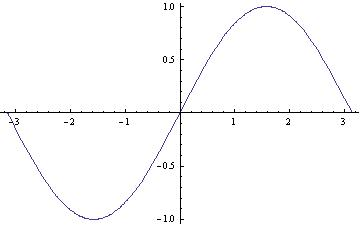
\includegraphics[height=2.5in, width=3.5in]{introduction/figures/sin_x.jpg}
\caption{Enjoyment and fun}
\end{figure}

Vestibulum ut urna eu turpis accumsan hendrerit. Mauris in mi sed eros auctor blandit. Nullam sit amet mauris vel eros aliquam pretium. Cras fermentum tortor. Sed egestas vulputate diam. Aenean sem dui, tincidunt a, ullamcorper eget, pharetra ac, tortor. In at sem vel elit bibendum convallis. Aenean ut enim vel leo malesuada dapibus. Etiam odio dolor, sollicitudin a, nonummy nec, tristique et, augue. Morbi ipsum. Aliquam venenatis. Proin orci. Duis sed quam eget turpis interdum feugiat.

\subsection{Hypothesis}  


Glossy prints of good reproducible quality, either black or white or color may be used. Photographs can be printed on 8 1/2$''$ x 11$''$ glossy finish paper, however, margin and page number requirements as stated above still apply for pages containing photographs. When attaching photographs to paper, double-sided tape may be used which causes the least amount of damage to the original paper.

The format of footnotes and the bibliography are to be prepared in accordance with standard practice in the field in which one is working. Documentation formatting style must be discussed with and accepted by the advisor. See further information on Reference Styles below.

The suggested typeface for dissertations is 10 to 12 point Arial. Other suggested fonts are Times New Roman and Helvetica. Script and italic fonts should not be used except as needed in the body of the paper. Consistency should be maintained throughout the paper, using the same font for all text, diagrams, etc. on all pages.

Electronic material, such as CDs and multimedia can accompany the dissertation. Each copy should be accompanied with a labeled CD. When bound, these are placed in an envelope in the back of the dissertation.  Oversized materials (pages greater than 8$''$ x 11$''$) can be included in the paper if necessary. Oversized pages should be folded so that 1$''$ on the left hand binding edge remains, allowing the page to be opened once the paper is bound.

The reference style used for formatting the paper must be confirmed with your department and advisor. Frequently used styles are the APA (American Psychological Association), MLA (Modern Language Association) and AMA (American Medical Association) styles. Style guides and manuals are available for each style. Page headers are not to be used.


\chapter{Methodology}
Three copies of the dissertation (1 original and 2 copies, either xerographic, photocopied, offset or letter quality printer) are to be supplied to the Library. In addition, an abstract independent of the document is to be supplied to the Library. The announcement for Ph.D. dissertation defense is to be given to The Office of the Registrar at least 1½ weeks prior to the defense. A sample defense announcement can be found in sample pages.

You must hand in your dissertation in person to the responsible person in the library. Dissertations cannot be mailed to the Library and cannot be handed in by another person.

\subsection*\normalsize\emph{Publication Agreement and Survey Forms}

The UMI Publication Agreement Form and a Survey of Earned Doctorates Form are submitted with the dissertation. The forms are available from Doris Oliver and online. Both forms must be completed and returned to Doris Oliver with the final dissertation. The UMI Publication Agreement Form includes the application form. This should be read, filled out and returned to Doris Oliver. The Survey of Earned Doctorates form is available online in two documents: the Survey of Earned Doctorates brochure and the Survey of Earned Doctorates form online.  UMI also provides a brochure on privacy as it relates to dissertations.

\subsection*\normalsize\emph{Use of Previously Published work in your dissertation}

If you are including previously published material as part of your dissertation, either as an appendix or as part of the body of your paper, you must obtain written permission from the publisher to have the work included as part of your paper.   Even if you are the author of the published material, you still must get permission from the publisher.    

Please view the dissertation specifications on the library website for information about UMI/Proquest's guide to copyright and copyright infringement. 

UMI/Proquest also includes information written by Kenneth Crews, a professor at Indiana University on the issue of copyright.  His work covers how to request permission from publishers, and sample permission letters.

\Large It is the responsibility of the student to ensure that all portions of their dissertation adhere to copyright law.  

\normalsize 


\chapter{Case Study}
All information about formatting a dissertation can be found on the library website at www.stevens.edu/library/services/phd.html.  Formatting information gets updated occasionally, so it is always good to check the requirements before submitting your dissertation.  

It is not required, but is strongly suggested that you make an appointment at the library to have the format of your dissertation reviewed before the final submission.  Dissertations can be rejected if they do not adhear to the formatting requirements.   

All information about formatting a dissertation can be found on the library website at www.stevens.edu/library/services/phd.html.  Formatting information gets updated occasionally, so it is always good to check the requirements before submitting your dissertation.  
It is not required, but is strongly suggested that you make an appointment at the library to have the format of your dissertation reviewed before the final submission.  Dissertations can be rejected if they do not adhear to the formatting requirements.   
All information about formatting a dissertation can be found on the library website at www.stevens.edu/library/services/phd.html.  Formatting information gets updated occasionally, so it is always good to check the requirements before submitting your dissertation.  

\begin{table}[htp]

\begin{center}
\begin{tabular}{|l|c|p{3.0in}|}
\hline
\multicolumn{3}{|c|}{Theoretical Dissertation Timeline}\\ \hline
Taskt&Time to Finish&Notes\\ \hline
Problem statement&10 hours&Initially very upbeat.\\ \hline
Research&3 days&Literature search to very previous studies.\\ \hline
Reformulation&4 hours&Presented and accepted by advisor\\ \hline
Research&20 days&Literature search to very previous  studies.\\ \hline
Experiments&14 days&Do some experiments and get results.\\ \hline
Format&1 day&Understand format guidelines for paper.\\ \hline
Write&years&Write the paper.\\ \hline
Revise&not too long&Proof read, etc.\\ \hline
Format&1-3 days&Verify correct report format is used.\\ \hline
See Library&1 hour&Meet with Doris to verify formatting.\\ \hline
Defend&1 day&Defend your research.\\ \hline
Revise&0 hours&It was perfect the first time.\\ \hline
Submit&1 day&Submit final dissertation to the library.\\ \hline
\end{tabular}
\end{center} 

\caption{Table of Tasks}\label{fig:erptsqfit}
\end{table}
It is not required, but is strongly suggested that you make an appointment at the library to have the format of your dissertation reviewed before the final submission.  Dissertations can be rejected if they do not adhear to the formatting requirements.   
All information about formatting a dissertation can be found on the library website at www.stevens.edu/library/services/phd.html.  Formatting information gets updated occasionally, so it is always good to check the requirements before submitting your dissertation.  
It is not required, but is strongly suggested that you make an appointment at the library to have the format of your dissertation reviewed before the final submission.  Dissertations can be rejected if they do not adhear to the formatting requirements.   
All information about formatting a dissertation can be found on the library website at www.stevens.edu/library/services/phd.html.  Formatting information gets updated occasionally, so it is always good to check the requirements before submitting your dissertation.  

It is not required, but is strongly suggested that you make an appointment at the library to have the format of your dissertation reviewed before the final submission.  Dissertations can be rejected if they do not adhear to the formatting requirements.   

\section{Further Analysis}  

\subsection*\normalsize\emph{Paper}
The original copy of the dissertation must be produced on good quality 8 1/2$''$ x 11$''$, 20 pound acid-free white paper. The paper should not be stapled, punched, bound, colored or printed on letterhead.

The two additional copies of the dissertation can be photocopied or produced on copier or laser paper.

\subsection*\normalsize\emph{Ink}
Black ink only is used to print your report.  If a graph or photograph contains color, that is fine. 

Latex is used to help in the printing of formulas.   The following formula would be difficult to reproduce in Microsoft Word: 
 \[
        \frac{d}{dx}\left( \int_{0}^{x} f(u)\,du\right)=f(x).
     \]

This Report was produced by LaTeX\footnote {\LaTeX\ is a fun typesetting program.} written by Barbara Arnett.  Barbara is not an expert with LaTeX, and anyone using LaTeX does not need to use this template.  It is simply provided to help with formatting, specifically with page numbers and images.  


%this subsection heading below will not show up in the table of contents.
\subsection*\normalsize\emph{Graphics} 

Graph paper may be used for original drawings, charts or illustrations. Original drawings may be in color or black and white, however, color is allowed for illustrations only; all text must appear in black. The original thesis must contain the original graphic or illustration, not a photocopy of the drawing, graphic or illustration.

If formulas and diagrams contain subscript and superscript characters, ensure they are large enough to read when printed in the final paper. 

\begin{figure}[htp]
\centering
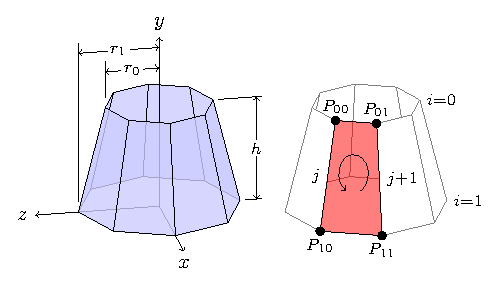
\includegraphics{casestudy/figures/3d-cone.pdf}
\caption{3D Cone}\label{fig:3d-cone}
\end{figure}

Photographs
Glossy prints of good reproducible quality, either black or white or color may be used. Photographs can be printed on 8 1/2$''$ x 11$''$ glossy finish paper, however, margin and page number requirements as stated above still apply for pages containing photographs. When attaching photographs to paper, double-sided tape may be used which causes the least amount of damage to the original paper. 

Graphics that are oriented in a landscape position must be done in a manner that retains the page numbering in the upper right hand corner, as shown in figure 3.2.  This can be difficult in Microsoft Word, but it is possible.  To do this in Microsoft Word, create a new section, change the page to landscape, and place the page number in a text box.  The text box then is rotated on the landscape page.    Then begin a new section and resume portrait orientation.

\begin{sidewaysfigure}
\centering
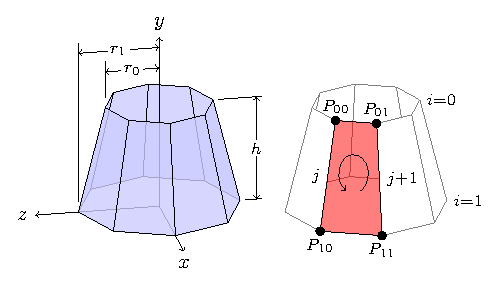
\includegraphics[height=5.0in, width=7.5in]{casestudy/figures/3d-cone.pdf}
\caption{This is an example of a landscape image within a page.  Note that the page number remains in the upper right hand corner of the page when the page is in the portrait position.}
\end{sidewaysfigure}

%!TEX root = ../thesis.tex
\chapter{Conclusions and Future Works}
\label{chap:chapter2}

\lipsum[2]

% At the end of each chapter
\newpage
%%%%% Appendices start %%%%%%%%%%%%%%%%
%% Comment out the following line if your thesis has no appendix
\addcontentsline{toc}{chapter}{Appendices}
\noindent \textbf{Appendices}
\appendix
\addcontentsline{toc}{section}{Appendix A}  %% removed \\
\noindent \textbf{Appendix A}
\vspace{12pt}

\noindent Appendices at the end of a dissertation are optional, and depend on the content of the dissertation. There can be one or more appendicies, however they should retain the page numbering requirements for dissertations.  Any concerns about the formatting of an appendix should be brought to Doris Oliver, who can direct you how to format your appendix if you have questions.

\begin{center}
\begin{tabular}{|l|c|p{3.0in}|}
\hline
\multicolumn{3}{|c|}{Theoretical Dissertation Timeline}\\ \hline
Taskt & Time to Finish & Notes\\ \hline
Problem statement & 10 hours & Initially very upbeat.\\ \hline
Research & 3 days&Literature search to very previous studies.\\ \hline
Reformulation&4 hours&Presented and accepted by advisor\\ \hline
Research&20 days&Literature search to very previous  studies.\\ \hline
Experiments&14 days&Do some experiments and get results.\\ \hline
Format&1 day&Understand format guidelines for paper.\\ \hline
Write&years&Write the paper.\\ \hline
Revise&not too long&Proof read, etc.\\ \hline
Format&1-3 days&Verify correct report format is used.\\ \hline
See Library&1 hour&Meet with Doris to verify formatting.\\ \hline
Defend&1 day&Defend your research.\\ \hline
Revise&0 hours&It was perfect the first time.\\ \hline
Submit&1 day&Submit final dissertation to the library.\\ \hline
\end{tabular}
\end{center}
\newpage

\addcontentsline{toc}{section}{Appendix B}  %% removed \\
\noindent \textbf{Appendix B}
\vspace{12pt}

\noindent Another one! Here is more text to go.
\newpage



%% Note: If your thesis has more than one appendix, NYU requires a "list of
%% appendices" page before the body of the thesis. I don't provide the tools
%% to create that here, so you're on your own for that one... Sorry.
%\addcontentsline{toc}{section}{Appendix B}  %% removed \\
\noindent \textbf{Appendix B}
\vspace{12pt}

\noindent Another one! Here is more text to go.
\newpage



%%%% Input bibliography file %%%%%%%%%%%%%%%
% %% Modified by Abdullah Khanfor for Stevens Institute of Technology PhD thesis format design guidelines 2019-2020
% NYU PhD thesis format. Original template created by José Koiller 2007--2008.
%% Updated by Anshul Vikram Pandey with new design guidelines. 2017-2018

%% Use the first of the following lines during production to
%% easily spot "overfull boxes" in the output. Use the second
%% line for the final version.
% \documentclass[12pt,draft,letterpaper]{report}
% \documentclass[12pt,letterpaper]{report}
\documentclass[12pt]{report}

%% Replace the title, name, advisor name, graduation date and dedication below with
%% your own. Graduation months must be January, May or September.
\newcommand{\thesistitle}{TITLE TO JUSTIFY YOUR PHD YEARS}
\newcommand{\thesisauthor}{Your Name}
\newcommand{\thesisadvisor}{Your Advisor's Name}
\newcommand{\thesisyear}{2020}
\newcommand{\thesisname}{Abdullah Khanfor}
\newcommand{\thesischairadvisor}{Dr. }    % this name prints on the title page as chairman and the abstract page as advisor
\newcommand{\committeenameA}{Dr. }
\newcommand{\committeenameB}{Dr. }
\newcommand{\committeenameC}{Dr. }
\newcommand{\thesisdepartment}{Systems Engineering}
\newcommand{\thesisdate}{November 22, 2020}
\newcommand{\thesistype}{dissertation}
\newcommand{\thesisdegree}{Doctor of Philosophy}
\newcommand{\graddate}{\the\year} % like 2020, 2019, no month or day should be written
\newcommand{\thesissigline}[1]{%
  \leftline{\hbox to 2.5in{}\hrulefill}
  \endgraf
  \vspace*{-18pt}
  \leftline{\hbox to 2.53in{}{#1}}}

%% If you do not want a dedication, scroll down and comment out
%% the appropriate lines in this file.
\newcommand{\thesisdedication}{To all the Ph.D. pursuing brave souls}

%% The following makes chapters and sections, but not subsections,
%% appear in the TOC (table of contents). Increase to 2 or 3 to
%% make subsections or subsubsections appear, respectively. It seems
%% to be usual to use the "1" setting, however.
\setcounter{tocdepth}{1}

%% Sectional units up to subsubsections are numbered. To number
%% subsections, but not subsubsections, decrease this counter to 2.
\setcounter{secnumdepth}{3}

% Setting a gap between page number and text block

%% This inputs your auxiliary file with \usepackage's and \newcommand's:
%% It is assumed that that file is called "definitions.tex".
\input{definitions}


%% Use the following commands, if desired, during production.
%% Comment them out for final version.
%\usepackage{layout} % defines the \layout command, see below
%\setlength{\hoffset}{-.75in} % creates a large right margin for notes and \showlabels

\pagestyle{fancy}
\fancyhf{}
% this prints a line under the header
\renewcommand{\headrulewidth}{0 pt}
%this prints a line under the footer
\renewcommand{\footrulewidth}{0 pt}
\fancyhead[RO]{}
\fancyhead[LO]{}
\fancyfoot[C]{}
\rhead{\thepage}

\fancypagestyle{plain}{%
\fancyhf{}
\rhead{\thepage}
}

%% Page layout (customized to letter paper and NYU requirements):
\setlength{\headheight}{20pt} 

%% Use the line below for official NYU version, which requires
%% double line spacing. For all other uses, this is unnecessary,
%% so the line can be commented out.
\onehalfspacing % requires package setspace, invoked above

%% Each of the following lines defines the \com command, which produces
%% a comment (notes for yourself, for instance) in the output file.
%% Example:    \com{this will appear as a comment in the output}
%% Choose (uncomment) only one of the three forms:
%\newcommand{\com}[1]{[/// {#1} ///]}       % between [/// and ///].
\newcommand{\com}[1]{\marginpar{\tiny #1}} % as (tiny) margin notes
%\newcommand{\com}[1]{}                     % suppress all comments.

%% Cross-referencing utilities. Use one or the other--whichever you prefer--
%% but comment out both lines for final version.
%\usepackage{showlabels}
%\usepackage{showkeys}
% \pagestyle{headings}

\begin{document}
%% Produces a test "layout" page, for "debugging" purposes only.
%% Comment out for final version.
%\layout % requires package layout (see above, on this same file)
%% Sets page numbering to "roman style" i, ii, iii, iv, etc:

%%%%%% Cover page %%%%%%%%%%%
%% Sets page numbering to "roman style" i, ii, iii, iv, etc:
\pagenumbering{roman}
\thispagestyle{empty}
\begin{center}
{
  {\thesistitle}
  \vspace{.15in}
  
    by
    
  \vspace{.15in}
  \thesisauthor
  
  \vspace{.15in}
  
 {A DISSERTATION}\\
  \vspace{.2in}
  \begin{spacing}{1}
    {Submitted to the Faculty of the Stevens Institute of Technology\\
    in partial fulfillment of the requirements for the degree of}
    \end{spacing}
  \vspace{.2in}
  
  {DOCTOR OF PHILOSOPHY}\\
  \vspace{1.0in}
  % for master thesis, change Chairman to Advisor
    \hfill 
    \begin{minipage}{80mm}
    \begin{spacing}{ }\noindent \rule{3.2in}{0.1mm}
        \thesisname, Candidate\\[3mm]
        \underline{ADVISORY COMMITTEE}\\[3mm]
        \noindent \rule{3.2in}{0.1mm}\\[-1.3mm]
        % for master thesis, change Chairman to Advisor
        {\thesischairadvisor}, Chairman  \hfill{Date}\\[2mm]
        {\noindent \rule{3.2in}{0.1mm}}\\[-1.3mm]
        {\committeenameA}        \hfill{Date}\\[2mm]
        {\noindent \rule{3.2in}{0.1mm}}\\[-1.3mm]
        {\committeenameB}        \hfill{Date}\\[2mm]
        {\noindent \rule{3.2in}{0.1mm}}\\[-1.3mm]
        {\committeenameC}        \hfill{Date}\\[2mm]
    \end{spacing}
  \end{minipage}
  \vfill
  
  {STEVENS INSTITUTE OF TECHNOLOGY\\
  \vspace{-0.05in}
  Castle Point on Hudson\\
  Hoboken, NJ 07030
  }
  % \vfill

  {\graddate}
}

\end{center}

\newpage



%%%%%%%%%%%%%% Microfilm / Publishing Page ProQuest %%%%%%%%%%%%%%%%%
% You can comment this section it is here to show you how it will appear when it submitted.
\thispagestyle{empty}
\begin{center}
ProQuest Number: XXXXXXXX

\vspace{.45in}

All rights reserved.

\vspace{.1in}

INFORMATION TO ALL USERS\\
The quality of this reproduction is dependent upon the quality of the copy submitted.
\vspace{.2in}

In the unlikely event hat  the author did not send a complete manuscript and there are missing pages, these will be  noted. Also ,if material had to be removed, a note will indicate the deletion.

\vspace{.1in}

\begin{figure}[H]
  \centering
  \includegraphics[width=200px]{misc/proquest-seeklogo.eps}
\end{figure}

\vspace{.1in}

ProQuest Number: XXXXXXXX

\vspace{.1in}

Published  by  ProQuest  LLC (\the\year).        Copyright of the Dissertation is held by the Author.

\vspace{.2in}

All rights reserved. This work is protected against  unauthorized copying under Title 17, United States Code Microform Edition {\textcopyright} ProQuest  LLC.

\vspace{.2in}

ProQuest LLC.\\
789 East Eisenhower Parkway\\
P.O. Box 1346\\
Ann Arbor, MI  48106-1346

\end{center}
\newpage

%%%%%% Copyrights page %%%%%%%%%%%
%
\setcounter{page}{2}
%% No numbering in the title page:
\thispagestyle{empty}
%
\begin{center}
{
  \vspace*{\fill}

  {\textcopyright} \graddate, \thesisname. All rights reserved.
}

\end{center}

\newpage
\doublespacing

%%%%%%%%%%%%%% Abstract %%%%%%%%%%%%%%%%%
\begin{center}
    {\thesistitle}\\ 
    {ABSTRACT}\\
    \vspace{.05in}
\end{center}
\addcontentsline{toc}{chapter}{Abstract}
\input{abstract}
\vspace{0.4in}
\begin{flushleft}
Author: \thesisname \\
Advisor: \thesischairadvisor \\
Date: \thesisdate \\
Department: \thesisdepartment \\
Degree: \thesisdegree \\
\end{flushleft}
\newpage

%%%%%%%%%%%%%% Dedication Page %%%%%%%%%%%%%%%%%
%% Comment out the following lines if you do not want to dedicate it is optional
\chapter*{Dedication}
\addcontentsline{toc}{chapter}{Dedication}
\strut \vspace{2in}
\begin{center}
``Most people are other people. Their thoughts are someone else's opinions, their lives a mimicry, their passions a quotation."
    \end{center}
    \vfill \strut
    \newpage
\newpage

%%%%%%%%%%%%%% Acknowledgements %%%%%%%%%%%%%%%%%
%% Comment out the following lines if you do not want to acknowledge
%% anyone's help...
\addcontentsline{toc}{chapter}{Acknowledgements}
\input{acknowledge}
\newpage

%%%% Table of Contents %%%%%%%%%%%%
\setcounter{tocdepth}{3} % To show a three level depth of sections

\tableofcontents

% \clearpage
% \pagestyle{headings}
\newpage

%%%%% List of Tables %%%%%%%%%%%%%
%% Comment out the following two lines if your thesis does not
%% contain any tables. The list of tables contains only
%% those tables included withing the "table" environment.
\listoftables\addcontentsline{toc}{chapter}{\listtablename}
\newpage

%%%%% List of Figures %%%%%%%%%%%%%
%% Comment out the following two lines if your thesis does not
%% contain any figures. The list of figures contains only
%% those figures included withing the "figure" environment.
\listoffigures\addcontentsline{toc}{chapter}{\listfigurename}
\newpage

%%%%% Body of thesis starts %%%%%%%%%%%%
\pagenumbering{arabic} % switches page numbering to arabic: 1, 2, 3, etc.

%% Introduction. If your thesis has no introduction, or chapter 1 is
%% meant to be the introduction, then comment out the lines below.
%% \section*{Introduction}\addcontentsline{toc}{section}{Introduction}
%\input{intro}

%%If your thesis has different "Parts", use commands such as the following:

\input{introduction/introduction}

\input{methodology/methodology}

\input{casestudy/casestudy}

\input{conclusion/conclusion}
%%%%% Appendices start %%%%%%%%%%%%%%%%
%% Comment out the following line if your thesis has no appendix
\addcontentsline{toc}{chapter}{Appendices}
\noindent \textbf{Appendices}
\appendix
\input{appendix/app1}
\input{appendix/app2}

%% Note: If your thesis has more than one appendix, NYU requires a "list of
%% appendices" page before the body of the thesis. I don't provide the tools
%% to create that here, so you're on your own for that one... Sorry.
%\input{app2}

%%%% Input bibliography file %%%%%%%%%%%%%%%
% \input{thesis}
\bibliographystyle{abbrv}
% Remember to remove the repated artificates/papers from the different files
\bibliography{biblio,introduction/introduction,methodology/methodology,casestudy/casestudy,conclusion/conclusion} % add intelligently
\newpage

%%%%%%%%%%%%%% Vita %%%%%%%%%%%%%%%%%
\section*{Vita}
\input{vita}
\newpage

\end{document}

\bibliographystyle{abbrv}
% Remember to remove the repated artificates/papers from the different files
\bibliography{biblio,introduction/introduction,methodology/methodology,casestudy/casestudy,conclusion/conclusion} % add intelligently
\newpage

%%%%%%%%%%%%%% Vita %%%%%%%%%%%%%%%%%
\section*{Vita}
%!TEX root = thesis.tex

Your vita goes here. This is usually a paragraph or two. Be careful about what you write here. :)

\lipsum[1]
\newpage

\end{document}

\bibliographystyle{abbrv}
% Remember to remove the repated artificates/papers from the different files
\bibliography{biblio,introduction/introduction,methodology/methodology,casestudy/casestudy,conclusion/conclusion} % add intelligently
\newpage

%%%%%%%%%%%%%% Vita %%%%%%%%%%%%%%%%%
\section*{Vita}
%!TEX root = thesis.tex

Your vita goes here. This is usually a paragraph or two. Be careful about what you write here. :)

\lipsum[1]
\newpage

\end{document}

\bibliographystyle{abbrv}
% Remember to remove the repated artificates/papers from the different files
\bibliography{biblio,introduction/introduction,methodology/methodology,casestudy/casestudy,conclusion/conclusion} % add intelligently
\newpage

%%%%%%%%%%%%%% Vita %%%%%%%%%%%%%%%%%
\section*{Vita}
%!TEX root = thesis.tex

Your vita goes here. This is usually a paragraph or two. Be careful about what you write here. :)

\lipsum[1]
\newpage

\end{document}
